% Preamble
% Document Configuration
\documentclass[a4paper, twoside, 11pt]{report}
\usepackage[margin=2cm]{geometry}
\usepackage[utf8]{inputenc}
\usepackage[english]{babel}
\usepackage{algorithm}
\usepackage{algorithmic}
\usepackage{amsmath}
\usepackage{csvsimple}
\usepackage{booktabs} % For better table formatting
\renewcommand{\baselinestretch}{1}
\setlength{\parskip}{1em}

% Reference Management
\usepackage[backend=biber, style=numeric, sorting=none]{biblatex}
\addbibresource{bibliography/bibliography.bib}

% Typography Improvements
\usepackage{setspace}
\usepackage{changepage}
\usepackage{emptypage}
\usepackage{csquotes}

% Graphics Support
\usepackage{graphicx}
\graphicspath{{images/}}

% Document Navigation
\usepackage{hyperref}
\hypersetup{
    colorlinks=true,
    linkcolor=black,
    filecolor=black,
    urlcolor=black, 
    citecolor=black
}

% Other packages
\usepackage{lipsum}
\usepackage{float}

% Document content begins here
\begin{document}

\pagenumbering{gobble}
\input{frontmatter/frontmatter-list.tex}

\cleardoublepage
{
    \setstretch{0}
    \tableofcontents
}

\cleardoublepage
{
    \setstretch{0}
    \listoffigures
}

\cleardoublepage
{
    \setstretch{0}
    \listoftables
}

\cleardoublepage
\pagenumbering{arabic}
\chapter{Introduction}

\section{Caching Problem}

Storing data in a faster storage medium to serve future requests faster for that data is a 
very common technique in computer science called caching. We will consider the problem 
of caching of pages of fixed size in a buffer pool of fixed size.

We call cache hit when the requested page is already in the cache, and cache fault or miss
when the requested page is not in the cache. Generally, the goal is to maximize the number
of cache hits.

When a page is accessed, and the buffer is full, we need to decide which page to evict
from the cache to make space for the new page. This is called the cache eviction policy,
and it is a crucial part of the caching problem.

The optimal cache eviction policy is to evict the page that will be requested the farthest
in the future \cite{lecture-notes-1} \cite{lecture-notes-2} \cite{article-for-belady-ref-1}.
But this is impractical in most cases, since it is generally impossible to predict how
far in the future a page will be requested.

Several cache eviction policies have been developed, which incorporate information
about recency and/or frequency of page requests to make eviction decisions, we will
discuss some of them in detail in the following chapters.

\section{Buffer Sharing in Multi-Tenant Caches}

In a multi-tenant environment, multiple tenants share the same buffer pool. Proper 
allocation of the buffer pool among tenants is crucial for the performance of each
tenant workload \cite{buffer-sharing-1}.

In this thesis, we will consider the problem of buffer sharing in multi-tenant caches,
where each tenant has completely different workloads, data of one tenant is completely
independent of the data of another tenant.

We mainly consider small number of tenants, since it is common in possible applications, 
experiments based on real data have 4 or 5 tenants, experiments on random data have up 
to 10 tenants, however, the proposed algorithms also work for larger number of tenants.

\subsection{Global, Static and Dynamic Buffer Allocation}

Some of the main approaches to buffer allocation in multi-tenant caches are:

\begin{enumerate}
    \item Global Buffer Allocation: All tenants share the same buffer pool, and the 
    buffer allocation is fixed. This approach is very simple and easy to implement,
    but it allows unlimited sharing of the buffer, and hence, it becoomes difficult to 
    guarantee the specified performance goal for individual tenants
    \cite{article-for-2level-forecasting} (Fig \ref{fig:figA-1}).
    \item Static Buffer Allocation: Each tenant has a fixed buffer size, and the buffer
    allocation is fixed. While straightforward to manage without sharing, a critical 
    downside of static caching is that it is hard to estimate the required amount of 
    the cache space in advance \cite{article-for-2level-forecasting} (Fig \ref{fig:figB-1}).
    \item Dynamic Buffer Allocation: The size of cache space for a tenant is adjusted 
    over time by monitoring performance. For this, it is critical to have good seasonality
    recommendations of cache sizes per tenant. Inadequate predictions will lead to the waste
    of resources or the failure of the performance guarantee \cite{article-for-2level-forecasting}
    There have been various studies to address this problem, such as based on the 
    approximation to concave functions \cite{approx-concave-functions} and a 
    learning-based prediction \cite{learning-based-prediction}, but it is still a 
    challenging problem to make accurate estimations of access patterns with an 
    acceptable error bound.
\end{enumerate}

\begin{figure}[H]
    \centering
    \begin{minipage}{0.4\textwidth}
        \centering
        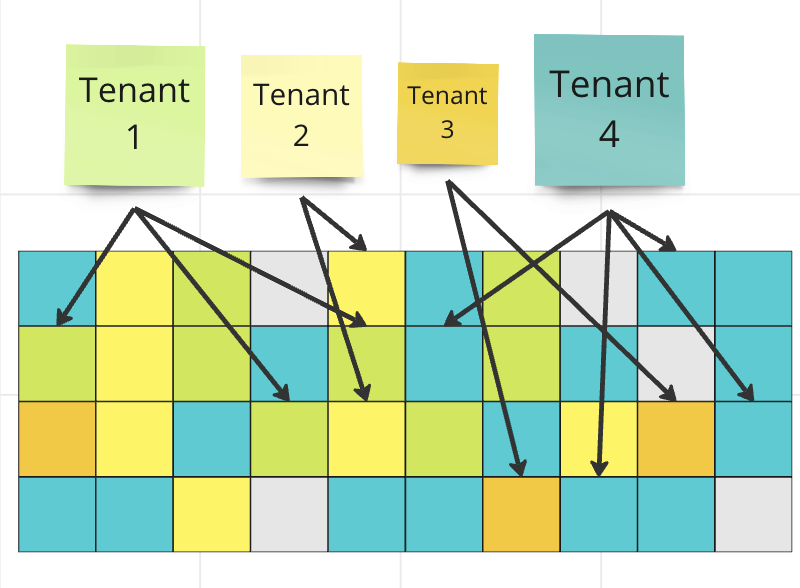
\includegraphics[width=\textwidth]{global_cache.png}
        \caption{Global Caching}
        \label{fig:figA-1}
    \end{minipage}
    \hfill
    \begin{minipage}{0.4\textwidth}
        \centering
        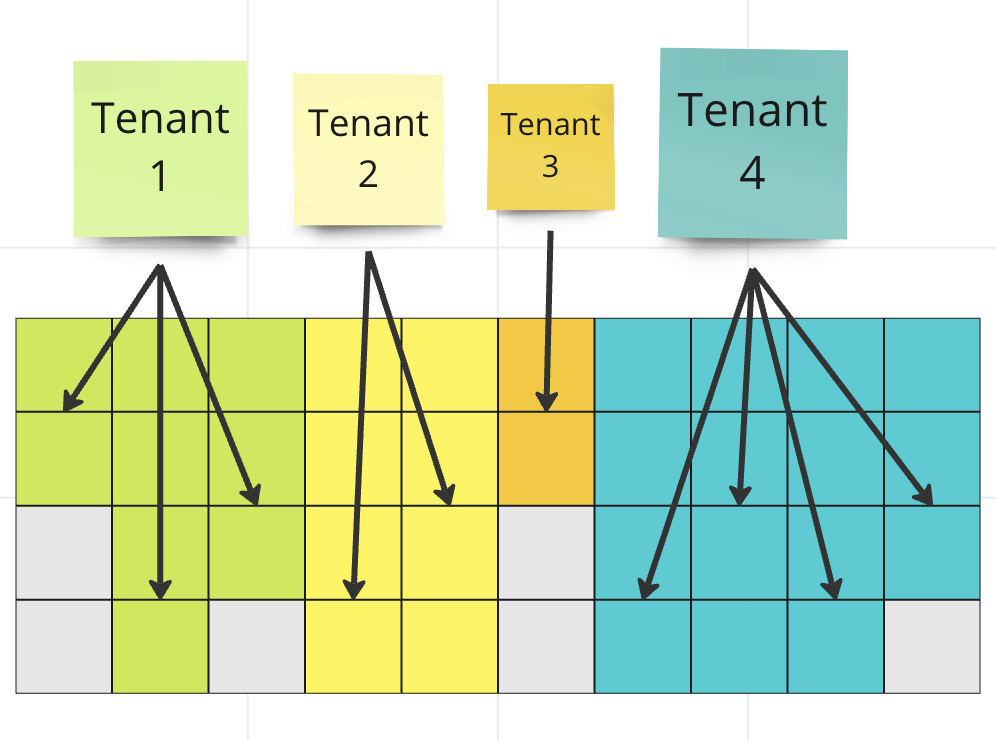
\includegraphics[width=\textwidth]{static_cache.png}
        \caption{Static Caching}
        \label{fig:figB-1}
    \end{minipage}
\end{figure}

The main case of study in this thesis is the dynamic buffer allocation, therefore our
caching policy will be adaptive to the buffer allocation of each tenant.

\subsection{Two level forecasting algorithm}

Since we are mainly interested in dynamic buffer allocation, caching problem in this
case can be seen as a two level forecasting problem. The first level is the seasonality
recommendation algorithm, which gives the buffer allocation of each tenant, and the
second level is the eviction policy, which makes eviction decisions based on the buffer
allocation.

The main focus of this thesis is on the eviction policy, for that, we will assume that
the buffer recommendations are given, and we will compare the performance of different
eviction policies.

While the recommendations are given, this does not mean that will have the cache problem
like single caches with fixed size, since the buffer allocation of each tenant is a 
recommendation that does not needs to be followed exactly, and it will also change
over time, therefore our eviction policy needs to be adaptive to the buffer allocation
of each tenant.

\subsection{Application to Multi-Tenant Relational Databases}

Relational database systems are widely used in many enterprises to store, manage and 
query data in applications in a structured way. Several commercial cloud relational
database services, such Google Cloud SQL \cite{google-cloud-sql}, Microsoft Azure SQL 
Database \cite{azure-sql}, and Oracle Cloud Database \cite{oracle-cloud} have emerged. 

In this cloud services, multi tenancy is crucial to increase consolidation and reduce
cost by sharing resources among tenants \cite{buffer-sharing-1}.

A database as a service (DaaS) provider would like to overbook the resources, i.e. 
promise more resources to tenants in aggregate than is physically available on the
machine, yet without affecting tenant performance. This is based on the observation 
that at any point in time some tenants on the machine are likely to use much fewer 
resources than they are promised. \cite{buffer-sharing-1} The main challenge is to 
allocate resources to tenants in a way that guarantees the performance of each tenant 
workload.

\section{Service Level Agreements and Hit Ratio Degradation}

In a multi-tenant environment, it is common to have service level agreements (SLAs)
or Quality of Service (QoS) requirements for each tenant. For example, in a cloud 
database service, a tenant may have promosed some amount of buffer space, and the
provider should guarantee a performance goal for the tenant.

The performance goal can be defined in terms of fault or hit ratio, like the fault
or hit ratio achieved if the tenant would had a dedicated cache of some promised size.
In a case where there is not a promised size like in the cloud environment, we can 
compare the achieved hit ratio with the hit ratio achieved by a tenant with a dedicated
cache of the size of the recommendation we have.

Metrics comparing the achieved hit ratio with the hit ratio of a dedicated cache have
been proposed in the literature, like the hit ratio degradation (HRD), as the difference 
in total hits, between the baseline and any scheme that assigns memory dynamically, 
normalized by the total memory accesses \cite{buffer-sharing-1} or other quality of 
service metrics like in \cite{learning-based-prediction}.

\section{Penalty Function Optimization}

We will consider the following penalty function to optimize:

$$
\sum_{t \in \text{Tenants}} \left( \frac{\text{Solution Cache faults}_t - \text{LRU Cache faults}_t}{\text{LRU Cache faults}_t} \right) ^2 \text{Priority}_t \left[\text{Solution Cache faults}_t \geq \text{LRU Cache faults}_t\right]
$$

In which, for each tenant $t$:
\begin{itemize}
    \item $\text{Solution Cache faults}_t$ is the number of cache faults of the eviction policy we are testing.
    \item $\text{LRU Cache faults}_t$ is the number of cache faults of the LRU eviction policy if we had a dedicated cache of some promised size.
    \item $\text{Priority}_t$ is the priority of the tenant, which can be defined in terms of the cost of a cache fault for the tenant, or the importance of the tenant. If there is no need to prioritize tenants, we can set $\text{Priority}_t = 1$ for all tenants, in case it is needed, priorities can be defined based on how importanat is for each tenant to achieve the promised hit ratio.
    \item The term in brackets is a condition so we only penalize the eviction policy if it has more cache faults than the isolated LRU eviction policy.
\end{itemize}

We normalize by the number of cache faults of the isolated LRU eviction policy, to make 
the penalty function independent of the number of tenants and the size of the cache, and to 
not prioritize tenants by the size of the access pattern.

We use squared ratio to penalize more the eviction policies that have a higher difference
in cache faults with the isolated LRU eviction policy, since we want to minimize the
difference in cache faults with the isolated LRU eviction policy, and smaller differences
are more tolerable.

This cost function was also used in ICPC 2023 Online Spring Challenge powered by Huawei: 
Buffer Sharing in Multi-Tenant Database Environment \cite{huawei-challenge}. Better results
were observed using this penalty function instead of using cache hits instead of faults.

Our goal is to minimize the penalty function, and we will compare the performance of
different eviction policies based on this penalty function.

\section{Research Question}

In multi-tenant caches, the main challenges are to allocate the buffer space among tenants
in a way that guarantees the performance of each tenant workload, and to design an eviction
policy that best satisfies the service level agreements for each tenant and does not waste
buffer space. 

Improving the cache performance in multi-tenant caches is interesting both for commercial
and research purposes, and it results in the main research question of this thesis:

\textit{How to design an eviction policy for multi-tenant caches that best satisfies 
the service level agreements for each tenant and does not waste buffer space?}

\section{Objectives}

To address the research question, the following objectives are proposed:

\begin{enumerate}
    \item Provide a clear overview of the multi-tenant caching problem.
    \item Describe the baseline algorithm with tenant selection policy and the cache eviction algorithm.
    \item Implement and describe different eviction policies, adapting them to the dynamic buffer size of each tenant.
    \item Perform experiments with real world data to compare the performance of different eviction policies.
    \item Analyze the results and propose improvements to the tenant selection and eviction policies.
\end{enumerate}

\section{Outline}

The outline for the rest of the thesis is as follows:

\begin{itemize}
    \item \textbf{Chapter 2: Algorithm Overview} - Will describe the base algorithm that we used, and discuss possible tenant selection and cache eviction policies.
    \item \textbf{Chapter 3: Experiments and Methodology} - Will describe the datasets we used, with data collection and processing part, and the performed experiments.
    \item \textbf{Chapter 4: Results} - Will present and analyze the results of the experiments, comparing different eviction policies.
    \item \textbf{Chapter 5: Conclusions and Recommendations} - Will summarize the results and propose recommendations for future work.
\end{itemize}

\cleardoublepage

\chapter{Algorithm Overview}

\section{Base Algorithm}

Let's describe the base algorithm of this thesis for multi-tenant caching, its detailed 
pseudcode is shown in Figure \ref{fig:base_algorithm}.

For each page access, the algorithm first checks if the page is in the cache,
in case it is, it returns the buffer location and the hit flag as true. It also 
updates the access history of the page in the cache eviction policy, for example,
for LRU, it moves the page to the top of the list (of that tenant).

If the page is not in the cache, the algorithm checks if there is available space
in the cache. If there is, it gets the first available buffer location and adds the
page to the cache. 

If there is no available space, the algorithm selects a page to evict from the cache 
using the tenant selection policy and the cache eviction policy. The algorithm then 
evicts the page and adds the new page to the cache.

Note that the tenant selection policy's responsibility is to select the tenant to evict
from the cache, each time a page needs to be evicted, for this, some metrics of the 
tenants can be used.

The cache eviction policy's responsibility is to manage the cache, including:
\begin{itemize}
    \item \textbf{UpdateAccessHistory}(\textit{page}, \textit{tenant}): Update the access history when a page is accessed.
    \item \textbf{AddPageToCache}(\textit{page}, \textit{tenant}, \textit{buffer\_location}): Add a page to the cache of a tenant in a specific buffer location.
    \item \textbf{EvictPage}(\textit{tenant\_to\_evict}): Evict a page from the cache of a tenant.
\end{itemize}

Each of the described tenant selection policies and cache eviction policies will implement
these functions, and the base algorithm will call them when needed.

Note that the base algorithm is a general dynamic multi-tenant cache algorithm that can 
be used with different tenant selection and cache eviction policies. The next sections 
will describe the tenant selection and cache eviction policies used with the base algorithm.

Another algorithm for dynamic multi-tenant buffer allocation was proposed in the 
literature in \cite{buffer-sharing-1}, a hybrid approach combining global and static 
buffer allocation was proposed in \cite{article-for-2level-forecasting}.

\begin{figure}[htbp]
    \centering
    \begin{minipage}{\linewidth}
    \begin{algorithm}[H]
        \caption{Base Algorithm to process each page access}
        \begin{algorithmic}
            \STATE \textbf{Input:} $(p, t)$ - The page id and tenant of the page to be accessed.
            \STATE \textbf{Output:} $(b, h)$ - The buffer location of the page accessed and whether it is a hit or not.
            \STATE
            \STATE $(\text{buffer\_location}, \text{is\_hit}) \leftarrow \text{GetPageLocationIfItIsInCache}(\text{page} = p, \text{tenant} = t)$
            \IF {$\text{is\_hit}$}
                \STATE $\text{CacheEvictionPolicy.UpdateAccessHistory}(\text{page} = p, \text{tenant} = t)$
                \RETURN $(b = \text{buffer\_location}, h = \textbf{true})$
            \ELSE
                \STATE \COMMENT {Page is not in cache, we need to find a place for it}
                \IF {There is available space in cache}
                    \STATE $\text{available\_location} \leftarrow \text{GetAvailableBufferLocation}()$ \COMMENT {Get the first available buffer location}
                    \STATE $\text{CacheEvictionPolicy.AddPageToCache(\text{page} = p, \text{tenant} = t, \text{available\_location})}$
                    \RETURN $(b = \text{available\_location}, h = \textbf{false})$
                \ELSE
                    \STATE \COMMENT {Cache is full, we need to evict a page}
                    \STATE $\text{tenant\_to\_evict} \leftarrow \text{TenantSelectionPolicy.GetTenantToEvict}()$
                    \STATE $\text{evicted\_page} \leftarrow \text{CacheEvictionPolicy.EvictPage}(\text{tenant\_to\_evict})$
                    \STATE $b \leftarrow \text{evicted\_page.buffer\_location}$
                    \STATE $\text{CacheEvictionPolicy.AddPageToCache}(\text{page} = p, \text{tenant} = t, \text{buffer\_location} = b)$
                    \RETURN $(b, h = \textbf{false})$
                \ENDIF
            \ENDIF
            \STATE
            \STATE \textbf{function} GetPageLocationIfItIsInCache(page, tenant):
            \STATE \hspace{\algorithmicindent} \textbf{if} page is in cache \textbf{then}
            \STATE \hspace{\algorithmicindent} \hspace{\algorithmicindent} \textbf{return} $(\text{page.buffer\_location}, \textbf{true})$
            \STATE \hspace{\algorithmicindent} \textbf{else}
            \STATE \hspace{\algorithmicindent} \hspace{\algorithmicindent} \textbf{return} $(\textbf{null}, \textbf{false})$
            \STATE \hspace{\algorithmicindent} \textbf{end if}
            \STATE \textbf{end function}
        \end{algorithmic}
    \end{algorithm}
    \caption{Base Algorithm}
    \label{fig:base_algorithm}
    \end{minipage}
\end{figure}
    

\section{Tenant Selection Policy}

The tenant selection policy is responsible for selecting the tenant
to evict from the cache when a page needs to be evicted.

In order to properly select the tenant to evict, the tenant selection policies will use 
some metrics of the tenants, such as the number of pages currently in the cache, 
the number of accesses, the number of hits, the number of faults. It is simple to 
keep track of these metrics with negligible overhead. In many applications, these 
metrics are already kept track of in the cache eviction policy, like in many DBMSs \cite{buffer-sharing-1}.

Other important metric that will allow us to better select the tenant to evict is 
the number of hits or faults if we had a cache of the promised size, or a cache 
$x\%$ higher than the recommendation in case there is no promised size, keeping track of 
this metrics requires additional overhead, like to simulate a LRU or other cache 
of the promised size for each tenant. Simulating a cache per tenant for selection 
purposes has been proposed and analysed in the literature in \cite{buffer-sharing-1}.

Many of the tenant selection policies described here will require aditional overhead 
metrics in order to work properly, in real applications, this overhead needs to be 
considered in comparison to the benefits of the eviction policy.

\subsection{Fault Ratio Policy}

Fault ratio policy comes from the idea that the tenant with the highest fault ratio
with respect to the fault ratio of the cache of the promised size (or size $x\%$ bigger than
the recommendation) should be evicted.

The evicted tenant $t$ is the one that minimizes the following formula:

$$
\left( \frac{\text{Solution Cache faults}_t - \text{LRU Cache faults}_t}{\text{LRU Cache faults}_t} \right) ^2 \text{Priority}_t \, \cdot \, \text{sgn}( \text{Solution Cache faults}_t - \text{LRU Cache faults}_t )
$$

Where:

\begin{itemize}
    \item $\text{Solution Cache faults}_t$ --- is the number of faults of the tenant in the cache of the promised size (or $x\%$ bigger than the recommendation).
    \item $\text{LRU Cache faults}_t$ --- is the number of faults of the tenant in a LRU cache of the promised size (or $x\%$ bigger than the recommendation).
    \item $\text{Priority}_t$ --- is the priority of the tenant.
    \item $\text{sgn}(x)$ --- is the sign function, returning $1$ if $x > 0$, $-1$ if $x < 0$ and $0$ if $x = 0$.
\end{itemize}

Note that we evict from the tenant that is performing the best in terms of our penalty
function, we use sign instead of condition to penalize by how much the tenant is performing
better than the LRU cache of the promised size, so we evict more from tenants that are
performing better.

This policy is a part of the policy proposed by Noé Weeks in \cite{noe-weeks-comments} for 
ICPC 2023 Online Spring Challenge powered by Huawei: Buffer Sharing in Multi-Tenant Database Environment \cite{huawei-challenge}.

Note that this tenant selection policy requires additional overhead to keep track of the
number of faults of the tenants in the cache of the promised size (or $x\%$ bigger than the recommendation),
so it needs to simulate an LRU cache for each tenant.

This policy can be modified to use as baseline algorithm to compare, the same cache algorithm
that will be used in the cache eviction policy, in order to use it as a quantitative measure 
of the impact of multi-tenancy on performance. We did not do this in this thesis, since
our penalty function is based on the LRU cache of the promised size.

\subsection{Hit Ratio Policy}

Hit ratio policy is very similar to the fault ratio policy, but instead of using the faults,
it uses the hits of the tenants in the cache of the promised size (or $x\%$ bigger than the recommendation).

The evicted tenant $t$ is the one that minimizes the following formula:

$$
\left( \frac{\text{LRU Cache hits}_t - \text{Solution Cache hits}_t}{\text{LRU Cache hits}_t} \right) ^2 \text{Priority}_t \, \cdot \, \text{sgn}( \text{LRU Cache hits}_t - \text{Solution Cache hits}_t )
$$

Where:

\begin{itemize}
    \item $\text{Solution Cache hits}_t$ --- is the number of hits of the tenant in the cache of the promised size (or $x\%$ bigger than the recommendation).
    \item $\text{LRU Cache hits}_t$ --- is the number of hits of the tenant in a LRU cache of the promised size (or $x\%$ bigger than the recommendation).
    \item $\text{Priority}_t$ --- is the priority of the tenant.
    \item $\text{sgn}(x)$ --- is the sign function, returning $1$ if $x > 0$, $-1$ if $x < 0$ and $0$ if $x = 0$.
\end{itemize}

This policy is very similar to the fault ratio policy, since more hits means less faults,
and we observed better results with the fault ratio policy, therefore we will use it more.

Like in the fault ratio policy, this policy requires additional overhead to keep track of the
number of hits of the tenants in the cache of the promised size (or $x\%$ bigger than the recommendation),
so it needs to simulate an LRU cache for each tenant.

This policy can also be modified to use as baseline algorithm to compare, the same cache algorithm
that will be used in the cache eviction policy, in order to use it as a quantitative measure
of the impact of multi-tenancy on performance.

\subsection{Fault Ratio with Cache Used Policy}

Fault ratio with cache used policy is a modification of the fault ratio policy, where we
divide by the ratio squared of the cache currently used by the tenant and the cache of the
promised size (or $x\%$ bigger than the recommendation).

The evicted tenant $t$ is the one that minimizes the following formula:

$$
\frac{ \left( \frac{\text{Solution Cache faults}_t - \text{LRU Cache faults}_t}{\text{LRU Cache faults}_t} \right) ^2 \text{Priority}_t \, \cdot \, \text{sgn}( \text{Solution Cache faults}_t - \text{LRU Cache faults}_t ) }{ \left( \frac{\text{Cache Used}_t}{\text{LRU Base Cache Size}_t} \right) ^2 }
$$

Where:

\begin{itemize}
    \item $\text{Solution Cache faults}_t$ --- is the number of faults of the tenant in the cache of the promised size (or $x\%$ bigger than the recommendation).
    \item $\text{LRU Cache faults}_t$ --- is the number of faults of the tenant in a LRU cache of the promised size (or $x\%$ bigger than the recommendation).
    \item $\text{Priority}_t$ --- is the priority of the tenant.
    \item $\text{sgn}(x)$ --- is the sign function, returning $1$ if $x > 0$, $-1$ if $x < 0$ and $0$ if $x = 0$.
    \item $\text{Cache Used}_t$ --- is the number of pages currently in the cache of the tenant.
    \item $\text{LRU Base Cache Size}_t$ --- is the size of the LRU cache of the promised size (or $x\%$ bigger than the recommendation) for the tenant.
\end{itemize}

The modification in this policy comes from the idea that if a tenant is using more cache
with respect to the cache of the promised size, it can match the base LRU performance 
better, so we can afford to evict more from this tenant, in the same way, if a tenant is
using less cache, it will be harder to match the base LRU performance, so we should evict
less from this tenant.

This policy requires same overhead as the fault ratio policy, since it needs to keep track
the same metrics plus the cache used by the tenants, which is a simple metric to keep track
of.

It can also be modified to use as baseline algorithm to compare, the same cache algorithm
that will be used in the cache eviction policy, in order to use it as a quantitative measure
of the impact of multi-tenancy on performance.

This policy showed the better results when we tried, therefore we will use it as the main 
tenant selection policy in this thesis, it was also used as the main tenant selection policy
by Noé Weeks \cite{noe-weeks-comments} in the ICPC 2023 Online Spring Challenge powered by Huawei: Buffer Sharing in
Multi-Tenant Database Environment \cite{huawei-challenge}.

\subsection{Naive Policy}

For the naive policy, we will evict from the tenant that its cache size is furthest
from the cache of the promised size (or $x\%$ bigger than the recommendation) (in ratio).

The evicted tenant $t$ is the one that minimizes the following formula:

$$
\frac{ \text{Cache Used}_t }{ \text{LRU Base Cache Size}_t }
$$

In case of a tie (each tenant has the number of pages in the cache with the same 
proportion to the recommendation), we will evict from the same tenant of the page that 
is being accessed.


In case of not changing recommendation, like in the case of comparing to the cache of
the promised size, this policy makes our algorithm behave like a static cache algorithm
for each tenant.

This policy requires no additional overhead, since it only needs to keep track of the
number of pages in the cache of the tenants.

\section{Cache Eviction Policy}

The cache eviction policy is responsible for managing the cache, including updating the
access history when a page is accessed, adding a page to the cache and evicting a page
from the cache.

The cache eviction policies will be used with the base algorithm, and they will implement
the following functions:

\begin{itemize}
    \item \textbf{UpdateAccessHistory}(\textit{page}, \textit{tenant}): Update the access history when a page is accessed.
    \item \textbf{AddPageToCache}(\textit{page}, \textit{tenant}, \textit{buffer\_location}): Add a page to the cache of a tenant in a specific buffer location.
    \item \textbf{EvictPage}(\textit{tenant\_to\_evict}): Evict a page from the cache of a tenant.
\end{itemize}

Note that the cache eviction policies need to be implemented in a different way with respect
to the single tenant cache problem, since here we can evict a page from one tenant, and 
use the freed space to add a page from another tenant, and the size assigned to each tenant
can change over time.

In the implementations, we will keep a separate structure of cache
for each tenant, like a separated linked list for each tenant in the case of LRU,
note that, however, buffer locations are shared between tenants, so we can evict a page
from one tenant and use the freed space to add a page from another tenant.

Since in this thesis we are focusing on the cache eviction and the tenant selection 
policies we will not keep cache items or pages themselves in the cache, we will just keep
the buffer location in the cache. 

Let's describe each of the cache eviction policy in detail in next sections.

\subsection{LRU}

Least Recently Used (Belady, 1966), is a cache eviction policy that evicts the page that was least
recently used, it comes from the assumption that the page that was least recently used is the
least likely to be used in the near future.

It was the was the algorithm of choice in the most cases until the early 80s \cite{2q-article},
and it is the cache eviction policy that has been studied the most and it is considered
the most predictable cache eviction policy \cite{lru-analysis-article}, and it never
replaces more than a factor of $B$ as many elements as the optimal offline algorithm, where $B$
is the size of the buffer \cite{lru-factor-b}. For example, LRU on a buffer of size $B$ will
never replace more than twice as many elements as the optimal or clairvoyant algorithm on a 
buffer of size $B/2$ \cite{2q-article}.

This eviction policy is usually implemented with a doubly linked list to keep track of the
access history of the pages and a hash table or array to keep track of the buffer location
of the pages, so it can process each page access in $O(1)$ time.

For LRU cache, we can implement each of the functions as follows:

\begin{itemize}
    \item \textbf{UpdateAccessHistory}(\textit{page}, \textit{tenant}): Move the page to the top of the list of the tenant.
    \item \textbf{AddPageToCache}(\textit{page}, \textit{tenant}, \textit{buffer\_location}): Add the page to the top of the list of the tenant.
    \item \textbf{EvictPage}(\textit{tenant\_to\_evict}): Evict the page from the bottom of the list of the tenant.
\end{itemize}

\begin{figure}[htbp]
    \centering
    \begin{minipage}{\linewidth}
    \begin{algorithm}[H]
        \caption{LRU Cache Eviction Policy}
        \begin{algorithmic}
            \STATE \textbf{function} UpdateAccessHistory(page, tenant):
            \STATE \hspace{\algorithmicindent} CacheList[tenant].\textbf{move\_to\_top}(CacheLocations[tenant][page])
            \STATE \hspace{\algorithmicindent} CacheLocations[tenant][page] = CacheList[tenant].\textbf{head}
            \STATE \textbf{end function}
            \STATE
            \STATE \textbf{function} AddPageToCache(page, tenant, buffer\_location):
            \STATE \hspace{\algorithmicindent} CacheList[tenant].\textbf{add\_to\_top}(page)
            \STATE \hspace{\algorithmicindent} CacheLocations[tenant][page] = CacheList[tenant].\textbf{head}
            \STATE \textbf{end function}

            \STATE
            \STATE \textbf{function} EvictPage(tenant\_to\_evict):
            \STATE \hspace{\algorithmicindent} page = CacheList[tenant\_to\_evict].\textbf{remove\_from\_tail}()
            \STATE \hspace{\algorithmicindent} CacheLocations[tenant][page] = \textbf{null}
            \STATE \hspace{\algorithmicindent} \textbf{return} page
            \STATE \textbf{end function}
        \end{algorithmic}
    \end{algorithm}
    \caption{LRU Cache Eviction Policy}
    \label{fig:lru}
    \end{minipage}
\end{figure}

CacheList is a doubly linked list per tenant, that keeps the pages in the cache,
in the order of the access history, the head of the list is the most recently used
page.

CacheLocations is a hash map or array that keeps the location of the pages in the cache,
so we can process each page access in $O(1)$ time.

\subsection{LFU}

Least Frequently Used (LFU) \cite{wikipedia-lfu} is a cache eviction policy that evicts
the page that was least frequently used, and if there is a tie (two or more pages have
the same frequency of use), it evicts the page that was least recently used. 
\cite{cache-management-algorithms-for-flexible-filesystems}

It is based on the idea that the pages accessed most frequently are the most likely 
to be accessed in the near future. 

When the probability distribution of the data access pattern is constant over time, LFU 
yields the highest performance \cite{lfu-highest-perf-zipf} \cite{lfu-highest-perf-inproc} \cite{tiny-lfu},
but in most practical workloads, the access frequency changes radically over time. For
example, in a video caching service; a video clip that is really popular on a 
given day might not be accessed a few days later. Hence, there is no point in 
keeping that item in cache once its popularity has faded just because it was once very 
popular \cite{tiny-lfu}.

In the ideal LFU, we would keep a counter of the number of accesses of each page,
even if the page is not in the cache, but this is not practical in real applications,
since it requires memory proportional to the number of pages accessed, therefore, in 
practice, frequency counter is kept in the cache, and it is forgotten when the page is
evicted \cite{wikipedia-lfu}.

Single tenant LFU can be implemented in $O(1)$ time \cite{o-1-lfu}, but it needs to keep
track of the frequency of the least frequently used page, and to keep this efficiently,
it relies on the fact that each time a page is evicted, a new page is added to the cache,
so it can update the frequency of the least frequently used page easily, but in multi-tenant
caching, we can evict a page from one tenant and add a page from another tenant, so we would
need to keep track of the frequency of the least frequently used page for each tenant in a
different way, which is not practical.

Due to this, we can not implement LFU in multi-tenant caching in $O(1)$ time, we would need
to use then a heap to keep track of the frequency of the pages, and a hash map or array to 
keep track of the locations of the pages, so we can implement LFU in multi-tenant caching 
in $O(\log n)$ time, where $n$ is the number of pages in the cache.

For LFU cache, we can implement each of the functions as follows:

\begin{itemize}
    \item \textbf{UpdateAccessHistory}(\textit{page}, \textit{tenant}): Increase the frequency of the page in the cache of the tenant, and update the heap.
    \item \textbf{AddPageToCache}(\textit{page}, \textit{tenant}, \textit{buffer\_location}): Add the page to the heap of the tenant, with the frequency of 1.
    \item \textbf{EvictPage}(\textit{tenant\_to\_evict}): Evict the page with the least frequency from the heap of the tenant.
\end{itemize}

\begin{figure}[htbp]
    \centering
    \begin{minipage}{\linewidth}
    \begin{algorithm}[H]
        \caption{LFU Cache Eviction Policy}
        \begin{algorithmic}
            \STATE \textbf{function} UpdateAccessHistory(page, tenant):
            \STATE \hspace{\algorithmicindent} pageInHeap = CacheLocations[tenant][page]
            \STATE \hspace{\algorithmicindent} pageInHeap.frequency += 1
            \STATE \hspace{\algorithmicindent} CacheLocations[tenant][page] = pageInHeap
            \STATE \hspace{\algorithmicindent} CacheHeaps[tenant].\textbf{heapify}(pageInHeap)
            \STATE \textbf{end function}
            \STATE
            \STATE \textbf{function} AddPageToCache(page, tenant, buffer\_location):
            \STATE \hspace{\algorithmicindent} pageInHeap = \textbf{new} PageInHeap(page = page, frequency = 1, buffer\_location = buffer\_location)
            \STATE \hspace{\algorithmicindent} CacheHeaps[tenant].\textbf{insert}(pageInHeap)
            \STATE \hspace{\algorithmicindent} CacheLocations[tenant][page] = pageInHeap
            \STATE \textbf{end function}

            \STATE
            \STATE \textbf{function} EvictPage(tenant\_to\_evict):
            \STATE \hspace{\algorithmicindent} page = CacheHeaps[tenant\_to\_evict].\textbf{extract\_min}()
            \STATE \hspace{\algorithmicindent} CacheLocations[tenant][page] = \textbf{null}
            \STATE \hspace{\algorithmicindent} \textbf{return} page
            \STATE \textbf{end function}
        \end{algorithmic}
    \end{algorithm}
    \caption{LFU Cache Eviction Policy}
    \label{fig:lfu}
    \end{minipage}
\end{figure}

CacheHeaps is a min heap per tenant, that keeps the pages in the cache, in the order of the
frequency of the pages, the root of the heap is the page with the least frequency.

CacheLocations is a hash map or array that keeps the location of the pages in the cache,
so we can process each page access in $O(1)$ time.

\subsection{LRU-2}

LRU-2 is a generalization of LRU, where LRU is LRU-1, and it is a special case of LRU-k, 
where $k = 2$. It is a cache eviction policy whose idea is to keep track of 
the second most recent refence of each page, using this information to estimate the 
inter-reference time of each page \cite{lru-k}.

Unlike LRU, LRU-2 is scan resistant, since it gives low priority to pages that have been 
scanned or to pages that belong to a big randomly accessed file \cite{2q-article}, and it 
does not suffer so much from access pattern changes like LFU, because of the correlated 
reference period \cite{lru-k}.

Correlated references are references that are close to each other in time, it has been 
shown that they are common in real workloads. They have been described in the literature 
\cite{lru-k} \cite{2q-article} \cite{lrfu-article}.

In order to handle the correlated references, and to be more resistant to access pattern 
changes, LRU-2 has a tunable parameter, the Correlated Reference Period, which is the
time window or number of references that are considered to be correlated.

LRU-2 evicts the page that has the smallest second-to-last access time, among the pages
that are not in the Correlated Reference Period.

In LRU-2, there is a need of keeping in memory a history of pages that are not in the 
cache, for example, if a page $p$ is accessed, it's recorded and stored in a buffer. If 
$p$ wasn't accessed recently enough to remember, its second to last access will be 0, 
and it will be evicted. To prevent cycling $p$ in and out of memory without recognizing 
its frequent use, we retain its access history for a while after its last access, this is 
called the Retained Information Period \cite{lru-k} \cite{2q-article}.

In the literature \cite{lru-k} LRU-2 is proposed to be implemented in an asynchronous way,
with separate processes or threads to handle pages that are no longer in the Correlated 
Reference Period, or pages that are no longer in the Retained Information Period, but in 
this thesis we will implement it in a synchronous, by defining the Correlated Reference
Period and the Retained Information Period in terms of the number of references.

Pages in the Correlated Reference Period will be handled in a FIFO list, pages in the cache
that are not in the Correlated Reference Period will be handled in a heap, since we need
to evict from these pages based on the second-to-last access time, pages in the Retained
Information Period could be handled with another heap to delete based on the second-to-last
access time, but to avoid additional overhead, since LRU-2 is already complex, we will
handle them in a FIFO list without affecting the performance of the algorithm too much
(note that using this, they will be evicted based on the time they were removed from the 
cache, but since this pages are not in the cache anymore, it will not affect much the performance
of the algorithm). 

For LRU-2 cache, we can implement each of the functions as follows:

\begin{itemize}
    \item \textbf{UpdateAccessHistory}(\textit{page}, \textit{tenant}): If the page is 
    in Correlated Reference Period, just update its last access time (do not update the 
    second-to-last access time, since it is a correlated reference), if the page is not 
    in the Correlated Reference Period, remove it from the heap, update its last and
    second-to-last access time, and add it to the front of the Correlated Reference 
    Period FIFO list, move last correlated page to the heap if needed.
    \item \textbf{AddPageToCache}(\textit{page}, \textit{tenant}, \textit{buffer\_location}): 
    Add the page to the front of the Correlated Reference Period FIFO list, move last 
    correlated page to the heap if needed.
    \item \textbf{EvictPage}(\textit{tenant\_to\_evict}): Evict the page on the top of 
    the heap (or from the FIFO list if the heap is empty), remove it and add it to the 
    Retained Information Period FIFO list, remove the last page from the Retained
    Information Period FIFO list if needed.
\end{itemize}

\begin{figure}[htbp]
    \centering
    \begin{minipage}{\linewidth}
    \begin{algorithm}[H]
        \caption{LRU-2 Cache Eviction Policy}
        \begin{algorithmic}
            \STATE \textbf{function} UpdateAccessHistory(page, tenant):
            \STATE \hspace{\algorithmicindent} \textbf{if} CRP\_Locations[tenant][page] != \textbf{null} \textbf{then}
            \STATE \hspace{\algorithmicindent} \hspace{\algorithmicindent} pageInCRP = CRP\_Locations[tenant][page]
            \STATE \hspace{\algorithmicindent} \hspace{\algorithmicindent} pageInCRP.last\_access = current\_time
            \STATE \hspace{\algorithmicindent} \textbf{else}
            \STATE \hspace{\algorithmicindent} \hspace{\algorithmicindent} page = HeapLocations[tenant][page]
            \STATE \hspace{\algorithmicindent} \hspace{\algorithmicindent} CacheHeaps[tenant].\textbf{remove}(page)
            \STATE \hspace{\algorithmicindent} \hspace{\algorithmicindent} HeapLocations[tenant][page] = \textbf{null}
            \STATE \hspace{\algorithmicindent} \hspace{\algorithmicindent} page.second\_to\_last\_access = page.last\_access
            \STATE \hspace{\algorithmicindent} \hspace{\algorithmicindent} page.last\_access = current\_time
            \STATE \hspace{\algorithmicindent} \hspace{\algorithmicindent} CRP\_List[tenant].\textbf{add\_to\_front}(page)
            \STATE \hspace{\algorithmicindent} \hspace{\algorithmicindent} CRP\_Locations[tenant][page] = CRP\_List[tenant].\textbf{head}
            \STATE \hspace{\algorithmicindent} \hspace{\algorithmicindent} \textbf{if} CRP\_List[tenant].\textbf{size}() $>$ CRP\_Size[tenant] \textbf{then}
            \STATE \hspace{\algorithmicindent} \hspace{\algorithmicindent} \hspace{\algorithmicindent} MoveLastPageInCRPToHeap(tenant)
            \STATE \hspace{\algorithmicindent} \hspace{\algorithmicindent} \textbf{end if}
            \STATE \hspace{\algorithmicindent} \textbf{end if}
            \STATE \textbf{end function}
            \STATE
            \STATE \textbf{function} AddPageToCache(page, tenant, buffer\_location):
            \STATE \hspace{\algorithmicindent} \textbf{if} RIP\_Locations[tenant][page] != \textbf{null} \textbf{then}
            \STATE \hspace{\algorithmicindent} \hspace{\algorithmicindent} pageInRIP = RIP\_Locations[tenant][page]
            \STATE \hspace{\algorithmicindent} \hspace{\algorithmicindent} second\_to\_last\_access = pageInRIP.last\_access
            \STATE \hspace{\algorithmicindent} \hspace{\algorithmicindent} RIP\_List[tenant].\textbf{remove}(pageInRIP)
            \STATE \hspace{\algorithmicindent} \hspace{\algorithmicindent} RIP\_Locations[tenant][page] = \textbf{null}
            \STATE \hspace{\algorithmicindent} \textbf{else}
            \STATE \hspace{\algorithmicindent} \hspace{\algorithmicindent} second\_to\_last\_access = 0
            \STATE \hspace{\algorithmicindent} \textbf{end if}
            \STATE \hspace{\algorithmicindent} pageInCRP = \textbf{new} PageInCRP(page = page, last\_access = current\_time, second\_to\_last\_access = second\_to\_last\_access, buffer\_location = buffer\_location)
            \STATE \hspace{\algorithmicindent} CRP\_List[tenant].\textbf{add\_to\_front}(pageInCRP)
            \STATE \hspace{\algorithmicindent} CRP\_Locations[tenant][page] = CRP\_List[tenant].\textbf{head}
            \STATE \hspace{\algorithmicindent} \textbf{if} CRP\_List[tenant].\textbf{size}() $>$ CRP\_Size[tenant] \textbf{then}
            \STATE \hspace{\algorithmicindent} \hspace{\algorithmicindent} MoveLastPageInCRPToHeap(tenant)
            \STATE \hspace{\algorithmicindent} \textbf{end if} 
            \STATE \textbf{end function}

            \STATE
            \STATE \textbf{function} EvictPage(tenant\_to\_evict):
            \STATE \hspace{\algorithmicindent} \textbf{if} \textbf{not} CacheHeaps[tenant\_to\_evict].\textbf{empty}() \textbf{then}
            \STATE \hspace{\algorithmicindent} \hspace{\algorithmicindent} page = CacheHeaps[tenant\_to\_evict].\textbf{extract\_min}()
            \STATE \hspace{\algorithmicindent} \hspace{\algorithmicindent} CRP\_Locations[tenant\_to\_evict][page] = \textbf{null}
            \STATE \hspace{\algorithmicindent} \hspace{\algorithmicindent} AddPageToRIPList(tenant\_to\_evict, page)
            \STATE \hspace{\algorithmicindent} \hspace{\algorithmicindent} \textbf{return} page
            \STATE \hspace{\algorithmicindent} \textbf{else}
            \STATE \hspace{\algorithmicindent} \hspace{\algorithmicindent} page = CRP\_List[tenant\_to\_evict].\textbf{extract\_from\_tail}()
            \STATE \hspace{\algorithmicindent} \hspace{\algorithmicindent} CRP\_Locations[tenant\_to\_evict][page] = \textbf{null}
            \STATE \hspace{\algorithmicindent} \hspace{\algorithmicindent} AddPageToRIPList(tenant\_to\_evict, page)
            \STATE \hspace{\algorithmicindent} \hspace{\algorithmicindent} \textbf{return} page
            \STATE \textbf{end function}
        \end{algorithmic}
    \end{algorithm}
    \caption{LRU-2 Cache Eviction Policy}
    \label{fig:lru-2}
    \end{minipage}
\end{figure}
\begin{figure}[htbp]
    \centering
    \begin{minipage}{\linewidth}
    \begin{algorithm}[H]
        \begin{algorithmic}
            \STATE \textbf{function} MoveLastPageInCRPToHeap(tenant):
            \STATE \hspace{\algorithmicindent} page = CRP\_List[tenant].\textbf{tail}
            \STATE \hspace{\algorithmicindent} CRP\_List[tenant].\textbf{remove}(page)
            \STATE \hspace{\algorithmicindent} CRP\_Locations[tenant][page] = \textbf{null}
            \STATE \hspace{\algorithmicindent} HeapLocations[tenant][page] = CacheHeaps[tenant].\textbf{insert}(page)
            \STATE \textbf{end function}
            \STATE
            \STATE \textbf{function} AddPageToRIPList(tenant, page):
            \STATE \hspace{\algorithmicindent} RIP\_List[tenant].\textbf{add\_to\_front}(page)
            \STATE \hspace{\algorithmicindent} RIP\_Locations[tenant][page] = RIP\_List[tenant].\textbf{head}
            \STATE \hspace{\algorithmicindent} \textbf{if} RIP\_List[tenant].\textbf{size}() $>$ RIP\_Size[tenant] \textbf{then}
            \STATE \hspace{\algorithmicindent} \hspace{\algorithmicindent} evictedPage = RIP\_List[tenant].\textbf{remove\_from\_tail}()
            \STATE \hspace{\algorithmicindent} \hspace{\algorithmicindent} RIP\_Locations[tenant][evictedPage] = \textbf{null}
            \STATE \hspace{\algorithmicindent} \textbf{end if}
            \STATE \textbf{end function}
        \end{algorithmic}
    \end{algorithm}
    \caption{Helper Functions for LRU-2 Cache Eviction Policy}
    \label{fig:lru-2-helper}
    \end{minipage}
\end{figure}

CRP\_List is a FIFO list per tenant, that keeps the pages in the cache that are in the
Correlated Reference Period, in the order of the access history.

CRP\_Locations is a hash map or array that keeps the location of the pages in the cache
that are in the Correlated Reference Period.

CacheHeaps is a min heap per tenant, that keeps the pages in the cache that are not in the
Correlated Reference Period, in the order of the second-to-last access time, the root of
the heap is the page with the smallest second-to-last access time.

HeapLocations is a hash map or array that keeps the location of the pages in the heap 
of each tenant's cache, that are not in the Correlated Reference Period.

RIP\_List is a FIFO list per tenant, that keeps the pages that are not in the cache anymore, 
but are in the Retained Information Period.

RIP\_Locations is a hash map or array that keeps the location of the pages in the Retained
Information Period.

\subsection{2Q}

2Q is a cache eviction policy that uses two queues, a FIFO queue for the
cold pages and a LRU queue for the hot pages.

Like LRU-2, 2Q is scan resistant, since it gives low priority to pages that have been
scanned or to pages that belong to a big randomly accessed file. It
is claimed to have similar performance to LRU-2, with less overhead \cite{2q-article}.

2Q algorithms maintains a FIFO queue A1in, with the pages that are cold, are in the cache
and were accessed recently, similar to the Correlated Reference Period in LRU-2.

It maintains another FIFO queue A1out, with the pages that are cold, but are not in 
the cache anymore, similar to the Retained Information Period in LRU-2.

It maintains a LRU queue Am, with the pages that are hot, which are all in the cache.

For 2Q cache, we can implement each of the functions as follows:

\begin{itemize}
    \item \textbf{UpdateAccessHistory}(\textit{page}, \textit{tenant}): If the page is 
    in Am queue, move it to the top of the Am queue, if the page is in A1in queue, do
    nothing since it is a correlated reference.
    \item \textbf{AddPageToCache}(\textit{page}, \textit{tenant}, \textit{buffer\_location}): If
    the page is in A1out queue, remove it from the A1out queue, and add it to the Am queue,
    otherwise, add it to the A1in queue.
    \item \textbf{EvictPage}(\textit{tenant\_to\_evict}): If the ratio of the number of pages
    in the A1in queue with respect to the number of pages in the cache of the tenant is bigger
    than a threshold, evict the page from the tail of the A1in queue, add it to the head of the
    A1out queue, and remove the page from the tail of the A1out queue if needed, otherwise, evict
    the page from the tail of the Am queue, and do not add it to the A1out queue since it has not
    been accessed in a while.
\end{itemize}

Note that each operation can be easily implemented in $O(1)$ time, and 2Q does not increase 
the overhead of simple LRU by more than a constant factor \cite{2q-article}.

\begin{figure}[htbp]
    \centering
    \begin{minipage}{\linewidth}
    \begin{algorithm}[H]
        \caption{2Q Cache Eviction Policy}
        \begin{algorithmic}
            \STATE \textbf{function} UpdateAccessHistory(page, tenant):
            \STATE \hspace{\algorithmicindent} \textbf{if} Am\_Locations[tenant][page] != \textbf{null} \textbf{then}
            \STATE \hspace{\algorithmicindent} \hspace{\algorithmicindent} Am\_List[tenant].\textbf{move\_to\_top}(page)
            \STATE \hspace{\algorithmicindent} \hspace{\algorithmicindent} Am\_Locations[tenant][page] = Am\_List[tenant].\textbf{head}
            \STATE \hspace{\algorithmicindent} \textbf{end if}
            \STATE \textbf{end function}
            \STATE
            \STATE \textbf{function} AddPageToCache(page, tenant, buffer\_location):
            \STATE \hspace{\algorithmicindent} \textbf{if} A1out\_Locations[tenant][page] != \textbf{null} \textbf{then}
            \STATE \hspace{\algorithmicindent} \hspace{\algorithmicindent} pageInA1out = A1out\_Locations[tenant][page]
            \STATE \hspace{\algorithmicindent} \hspace{\algorithmicindent} A1out\_List[tenant].\textbf{remove}(pageInA1out)
            \STATE \hspace{\algorithmicindent} \hspace{\algorithmicindent} A1out\_Locations[tenant][page] = \textbf{null}
            \STATE \hspace{\algorithmicindent} \hspace{\algorithmicindent} Am\_List[tenant].\textbf{add\_to\_front}(page)
            \STATE \hspace{\algorithmicindent} \hspace{\algorithmicindent} Am\_Locations[tenant][page] = Am\_List[tenant].\textbf{head}
            \STATE \hspace{\algorithmicindent} \textbf{else}
            \STATE \hspace{\algorithmicindent} \hspace{\algorithmicindent} A1in\_List[tenant].\textbf{add\_to\_front}(page)
            \STATE \hspace{\algorithmicindent} \hspace{\algorithmicindent} A1in\_Locations[tenant][page] = A1in\_List[tenant].\textbf{head}
            \STATE \hspace{\algorithmicindent} \textbf{end if}
            \STATE \textbf{end function}

            \STATE
            \STATE \textbf{function} EvictPage(tenant\_to\_evict):
            \STATE \hspace{\algorithmicindent} TenantCacheUsed = A1in\_Size[tenant\_to\_evict].\textbf{size}() + Am\_Size[tenant\_to\_evict].\textbf{size}()
            \STATE \hspace{\algorithmicindent} \textbf{if} (A1in\_List[tenant\_to\_evict].\textbf{size}() / TenantCacheUsed $>$ A1in\_Threshold \textbf{and not} A1in\_List[tenant\_to\_evict].\textbf{empty}()) \textbf{or} Am\_List[tenant\_to\_evict].\textbf{empty}() \textbf{then}
            \STATE \hspace{\algorithmicindent} \hspace{\algorithmicindent} page = A1in\_List[tenant\_to\_evict].\textbf{remove\_from\_tail}()
            \STATE \hspace{\algorithmicindent} \hspace{\algorithmicindent} AddPageToA1OutList(tenant\_to\_evict, page)
            \STATE \hspace{\algorithmicindent} \hspace{\algorithmicindent} \textbf{return} page
            \STATE \hspace{\algorithmicindent} \textbf{else}
            \STATE \hspace{\algorithmicindent} \hspace{\algorithmicindent} page = Am\_List[tenant\_to\_evict].\textbf{remove\_from\_tail}()
            \STATE \hspace{\algorithmicindent} \hspace{\algorithmicindent} Am\_Locations[tenant\_to\_evict][page] = \textbf{null}
            \STATE \hspace{\algorithmicindent} \hspace{\algorithmicindent} \textbf{return} page
            \STATE \hspace{\algorithmicindent} \textbf{end if}
            \STATE \textbf{end function}
        \end{algorithmic}
    \end{algorithm}
    \begin{algorithm}[H]
        \begin{algorithmic}
            \STATE \textbf{function} AddPageToA1OutList(tenant, page):
            \STATE \hspace{\algorithmicindent} \hspace{\algorithmicindent} A1out\_List[tenant].\textbf{add\_to\_front}(page)
            \STATE \hspace{\algorithmicindent} \hspace{\algorithmicindent} A1out\_Locations[tenant][page] = A1out\_List[tenant].\textbf{head}
            \STATE \hspace{\algorithmicindent} \hspace{\algorithmicindent} \textbf{if} A1out\_List[tenant].\textbf{size}() / TenantCacheSizeRecommendation[tenant] $>$ A1out\_Threshold \textbf{then}
            \STATE \hspace{\algorithmicindent} \hspace{\algorithmicindent} \hspace{\algorithmicindent} evictedPage = A1out\_List[tenant].\textbf{remove\_from\_tail}()
            \STATE \hspace{\algorithmicindent} \hspace{\algorithmicindent} \hspace{\algorithmicindent} A1out\_Locations[tenant][evictedPage] = \textbf{null}
            \STATE \hspace{\algorithmicindent} \hspace{\algorithmicindent} \textbf{end if}
            \STATE \textbf{end function}
        \end{algorithmic}
    \end{algorithm}
    \caption{2Q Cache Eviction Policy}
    \label{fig:2q}
    \end{minipage}
\end{figure}

\newpage

A1in\_List is a FIFO list per tenant, that keeps the pages in the cache that are cold, are
in the cache and were accessed recently, similar to the Correlated Reference Period in LRU-2.

A1in\_Locations is a hash map or array that keeps the location of the pages in A1in\_List.  

A1out\_List is a FIFO list per tenant, that keeps the pages in the cache that are cold, but
are not in the cache anymore, similar to the Retained Information Period in LRU-2.

A1out\_Locations is a hash map or array that keeps the location of the pages in A1out\_List.

Am\_List is a doubly linked list per tenant, that keeps the pages in the cache that are hot,
which are all in the cache.

Am\_Locations is a hash map or array that keeps the location of the pages in the cache of each
tenant.

A1in\_Treshold is a tunable parameter that defines the ratio of the number of pages in the A1in
queue with respect to the number of pages in the cache, it is claimed that 0.25 works well in
most cases \cite{2q-article}.

A1out\_Treshold is a tunable parameter that defines the ratio of the number of pages in the A1out
queue with respect to the cache size recommendation, it is claimed that 0.5 works well in most
cases \cite{2q-article}.

TenantCacheSizeRecommendation is the cache size recommendation for each tenant.

\subsection{MQ}

It has been shown that a good cache eviction policy should satisfy the following properties:

\begin{enumerate}
    \item \textbf{Minimal lifetime:} Warm pages should not be evicted too soon (for 
    example, MRU does not satisfy this property).
    \item \textbf{Frequency-based priority:} Pages should be prioritized based on their 
    frequencies. (LFU satisfies this property, but LRU does not).
    \item \textbf{Temporal frequency:} Pages accessed frequently in the past, but not 
    accessed in a relatively long time, should be evicted (LRU satisfies this property, 
    but LFU does not).
\end{enumerate}

Multi-Queue (MQ) is a cache eviction policy that aims to satisfy all these properties \cite{mq-article}
by maintaining pages with different access frequencies in the cache for different time periods.

It uses multiple LRU queues $Q_0, Q_1, \ldots, Q_{m-1}$, where $m$ is a tunable parameter, pages in $Q_j$
have a longer lifetime than pages in $Q_{i}$ for $i < j$ \cite{mq-article}.

MQ uses a memory buffer $Q_{out}$ to remember recently evicted pages for a period of time, similarly to
2Q algorithm \cite{2q-article} or the Retained Information Period in LRU-2. It is handled by a 
FIFO queue of limited size.

On a cache hit to page $p$, $p$ is first removed from current LRU queue, and then added to 
$Q_{\text{num\_queue(frequency(p))}}$, that is, we insert it on a queue based on the frequency of the page,
for example, $\text{num\_queue(f)}$ can be defined as $\log_2(f)$, where $f$ is the frequency of the page.
Then the $8$th access of a page will promote it from $Q_2$ to $Q_3$ \cite{mq-article}.

In order to evict pages that were accessed frequently in the past, but not accessed in a relatively long time,
MQ demotes pages to lower queues after a certain period of time $lifeTime$ after the last access, this is
a tunable parameter \cite{mq-article}.

In order to handle demotion, every time a page enters a queue, its value $expireTime$ is set to $currentTime + lifeTime$.
After each access, queues are adjusted, if the $expireTime$ of a queue's tail page is less than the current time, the page
is moved to the next lower queue, and the $expireTime$ is updated to $currentTime + lifeTime$.

Here time is measured as logical time, that is, the number of accesses, in order to isolate 
this parameters from multi-tenancy, we will keep a separate logical time for each tenant \cite{mq-article}.

For MQ cache, we can implement each of the functions as follows:

\begin{itemize}
    \item \textbf{UpdateAccessHistory}(\textit{page}, \textit{tenant}): Remove the page from the
    current LRU queue, update its frequency, and add it to the corresponding LRU queue based on the
    frequency of the page using $\text{num\_queue}(\text{frequency}(page))$.
    \item \textbf{AddPageToCache}(\textit{page}, \textit{tenant}, \textit{buffer\_location}): If 
    $page$ is in $Q_{out}$, remove it from $Q_{out}$, and add it to the corresponding LRU queue based
    on the frequency of the page using $\text{num\_queue}(\text{frequency}(page))$, otherwise, add it
    to $Q_0$.
    \item \textbf{EvictPage}(\textit{tenant\_to\_evict}): Evict the page from the tail of the LRU queue with the
    smallest index that is not empty, and add it to $Q_{out}$, remove the page from the tail of $Q_{out}$ if needed.
\end{itemize}

Each operation can be implemented in $O(1)$ or $O(q)$ time, where $q$ is the number of LRU queues,
this number is a tunable parameter, and it is usally very small, in most cases less than 10 \cite{mq-article}.

To handle the demotion of pages, the method \textbf{AdjustQueues} will be called for each tenant after each access.

\begin{figure}[htbp]
    \centering
    \begin{minipage}{\linewidth}
    \begin{algorithm}[H]
        \caption{MQ Cache Eviction Policy}
        \begin{algorithmic}
            \STATE \textbf{function} UpdateAccessHistory(page, tenant):
            \STATE \hspace{\algorithmicindent} (pageInLRUQueue, currentQueue) = LRUQueueLocations[tenant][page]
            \STATE \hspace{\algorithmicindent} LRUQueues[tenant][currentQueue].\textbf{remove}(pageInLRUQueue)
            \STATE \hspace{\algorithmicindent} page.frequency = page.frequency + 1
            \STATE \hspace{\algorithmicindent} queueToAdd = \textbf{num\_queue}(page.frequency)
            \STATE \hspace{\algorithmicindent} page.expireTime = currentTime[tenant] + lifeTime[tenant]
            \STATE \hspace{\algorithmicindent} LRUQueues[tenant][queueToAdd].\textbf{add\_to\_top}(page)
            \STATE \hspace{\algorithmicindent} LRUQueueLocations[tenant][page] = (LRUQueues[tenant][queueToAdd].\textbf{head}, queueToAdd)
            \STATE \textbf{end function}
            \STATE
            \STATE \textbf{function} AddPageToCache(page, tenant, buffer\_location):
            \STATE \hspace{\algorithmicindent} \textbf{if} Qout\_Locations[tenant][page] != \textbf{null} \textbf{then}
            \STATE \hspace{\algorithmicindent} \hspace{\algorithmicindent} pageInQout = Qout\_Locations[tenant][page]
            \STATE \hspace{\algorithmicindent} \hspace{\algorithmicindent} pageFrequency = page.frequency + 1
            \STATE \hspace{\algorithmicindent} \hspace{\algorithmicindent} Qout\_List[tenant].\textbf{remove}(pageInQout)
            \STATE \hspace{\algorithmicindent} \hspace{\algorithmicindent} Qout\_Locations[tenant][page] = \textbf{null}
            \STATE \hspace{\algorithmicindent} \textbf{else}
            \STATE \hspace{\algorithmicindent} \hspace{\algorithmicindent} pageFrequency = 1
            \STATE \hspace{\algorithmicindent} \textbf{end if}
            \STATE \hspace{\algorithmicindent} queueToAdd = \textbf{num\_queue}(pageFrequency)
            \STATE \hspace{\algorithmicindent} page.expireTime = currentTime[tenant] + lifeTime[tenant]
            \STATE \hspace{\algorithmicindent} LRUQueues[tenant][queueToAdd].\textbf{add\_to\_top}(page)
            \STATE \hspace{\algorithmicindent} LRUQueueLocations[tenant][page] = (LRUQueues[tenant][queueToAdd].\textbf{head}, queueToAdd)
            \STATE \textbf{end function}

            \STATE
            \STATE \textbf{function} EvictPage(tenant\_to\_evict):
            \STATE \hspace{\algorithmicindent} \textbf{for} $i = 0$ \textbf{to} $q - 1$ \textbf{do}
            \STATE \hspace{\algorithmicindent} \hspace{\algorithmicindent} \textbf{if} \textbf{not} LRUQueues[tenant\_to\_evict][i].\textbf{empty}() \textbf{then}
            \STATE \hspace{\algorithmicindent} \hspace{\algorithmicindent} \hspace{\algorithmicindent} pageToEvict = LRUQueues[tenant\_to\_evict][i].\textbf{remove\_from\_tail}()
            \STATE \hspace{\algorithmicindent} \hspace{\algorithmicindent} \hspace{\algorithmicindent} LRUQueueLocations[tenant\_to\_evict][pageToEvict] = \textbf{null}
            \STATE \hspace{\algorithmicindent} \hspace{\algorithmicindent} \hspace{\algorithmicindent} AddPageToQout(tenant\_to\_evict, pageToEvict)
            \STATE \hspace{\algorithmicindent} \hspace{\algorithmicindent} \textbf{return} pageToEvict
            \STATE \textbf{end function}
        \end{algorithmic}
    \end{algorithm}
    \caption{MQ Cache Eviction Policy}
    \label{fig:mq}
    \end{minipage}
\end{figure}

\newpage

\begin{figure}[htbp]
    \centering
    \begin{minipage}{\linewidth}
    \begin{algorithm}[H]
        \begin{algorithmic}
            \STATE \textbf{function} AddPageToQout(tenant, page):
            \STATE \hspace{\algorithmicindent} Qout\_List[tenant].\textbf{add\_to\_front}(page)
            \STATE \hspace{\algorithmicindent} Qout\_Locations[tenant][page] = Qout\_List[tenant].\textbf{head}
            \STATE \hspace{\algorithmicindent} \textbf{if} A1out\_List[tenant].\textbf{size}() / TenantCacheSizeRecommendation[tenant] $>$ A1out\_Threshold \textbf{then}
            \STATE \hspace{\algorithmicindent} \hspace{\algorithmicindent} evictedPage = Qout\_List[tenant].\textbf{remove\_from\_tail}()
            \STATE \hspace{\algorithmicindent} \hspace{\algorithmicindent} Qout\_Locations[tenant][evictedPage] = \textbf{null}
            \STATE \hspace{\algorithmicindent} \textbf{end if}
            \STATE \textbf{end function}
            \STATE 
            \STATE \textbf{function} AdjustQueues(tenant, was\_accessed\_now):
            \STATE \hspace{\algorithmicindent} \textbf {if} was\_accessed\_now \textbf{then}
            \STATE \hspace{\algorithmicindent} \hspace{\algorithmicindent} currentTime[tenant] = currentTime[tenant] + 1
            \STATE \hspace{\algorithmicindent} \textbf{end if}
            \STATE \hspace{\algorithmicindent} \textbf{for} $i = 1$ \textbf{to} $q - 1$ \textbf{do}
            \STATE \hspace{\algorithmicindent} \hspace{\algorithmicindent} tailPage = LRUQueues[tenant][i].\textbf{tail}
            \STATE \hspace{\algorithmicindent} \hspace{\algorithmicindent} \textbf{if} tailPage.expireTime $<$ currentTime[tenant] \textbf{then}
            \STATE \hspace{\algorithmicindent} \hspace{\algorithmicindent} \hspace{\algorithmicindent} LRUQueues[tenant][i].\textbf{remove}(tailPage)
            \STATE \hspace{\algorithmicindent} \hspace{\algorithmicindent} \hspace{\algorithmicindent} tailPage.expireTime = currentTime[tenant] + lifeTime[tenant]
            \STATE \hspace{\algorithmicindent} \hspace{\algorithmicindent} \hspace{\algorithmicindent} LRUQueues[tenant][i - 1].\textbf{add\_to\_front}(tailPage)
            \STATE \hspace{\algorithmicindent} \hspace{\algorithmicindent} \hspace{\algorithmicindent} LRUQueueLocations[tenant][tailPage] = (LRUQueues[tenant][i - 1].\textbf{head}, i - 1)
            \STATE \hspace{\algorithmicindent} \hspace{\algorithmicindent} \textbf{end if}
            \STATE \hspace{\algorithmicindent} \textbf{end for}
            \STATE \textbf{end function}
        \end{algorithmic}
    \end{algorithm}
    \caption{Helper Functions for MQ Cache Eviction Policy}
    \label{fig:mq-helper}
    \end{minipage}
\end{figure}

LRUQueues is an array of doubly linked lists per tenant, that keeps the pages in the cache,
each list is an LRU queue, and the index of the list is the queue number.

LRUQueueLocations is a hash map or array that keeps the location of the pages in the LRU queues,
each location is a tuple with the location in the LRU queue and the queue number.

Qout\_List is a FIFO list per tenant, that keeps the pages in the cache that are not in the cache
anymore, but were recently evicted.

Qout\_Locations is a hash map or array that keeps the location of the pages in the Qout list.

num\_queue is a function that returns the queue number based on the frequency of the page,
it is usually defined as $\log_2(f)$, where $f$ is the frequency of the page \cite{mq-article}.

TenantCacheSizeRecommendation is the cache size recommendation for each tenant.

A1out\_Treshold is a tunable parameter that defines the ratio of the number of pages in the A1out
queue with respect to the cache size recommendation.

lifeTime is a tunable parameter that defines the time a page can stay in a queue without being accessed,
it is separate for each tenant, and it is usually defined as a fraction of the cache size recommendation.

currentTime is a logical time that is incremented after each access, it is separate for each tenant.

\subsection{LIRS}

Low Inter-reference Recency Set (LIRS) is a cache eviction policy that uses the number 
of references between the last two references to a page, called Inter-reference recency
(IRR) to split the pages in the cache into two sets, the Low IRR set (LIRS) and the 
High IRR set (HIRS) \cite{lirs-article}.

It assumes that if the IRR of a page is large, the next IRR will be large as well. Following
this assumption, blocks with large IRRs are chosen for eviction \cite{lirs-article}.

LIRS is scan resistant, considers not only the recency of the page, but also the
frequency, using the IRR and and it does not suffer too much from access pattern changes.

The algorithm dinamically and responsively distinguishes between low and high IRR \cite{lirs-article}.

A small portion on the cache is used for the HIR pages, the HIR pages that are in the cache
are called Resident HIR pages. Some HIR blocks that were evicted recently, could be kept 
recorded for some time, these are called Non-Resident HIR pages.

The LIRS list is maintained, it contains all the LIRS pages, and some of the HIR pages 
which can be resident or not (Fig \ref{fig:lirs_and_hirs_lists}), it is maintained in such a 
way that the last page of the LIRS list is a LIRS page. In order to maintain this property,
the LIRS list is pruned after each operation (the last pages that are not LIRS pages are removed)
\cite{lirs-article}.

HIRS list contains the resident HIR pages, regardless if they are in the LIRS list or not 
(Fig \ref{fig:lirs_and_hirs_lists}).

When a page is accessed, if it was in the LIRS list, it will become a LIRS page (if it was not)
and it will be moved to the front of the LIRS list. If it was not in the LIRS list, it will be
added to the front of the HIRS and LIRS lists, but marked as a HIR page.

A tunable parameter \textbf{LIRS\_Threshold} defines the ratio of the number of
LIRS pages with respect to the cache size, after each operation, if the number of LIRS pages is
bigger than this threshold, the last page of the LIRS list will be moved to the HIR list, and
the LIRS list will be pruned.

\begin{figure}[H]
    \centering
    \begin{minipage}{0.5\textwidth}
        \centering
        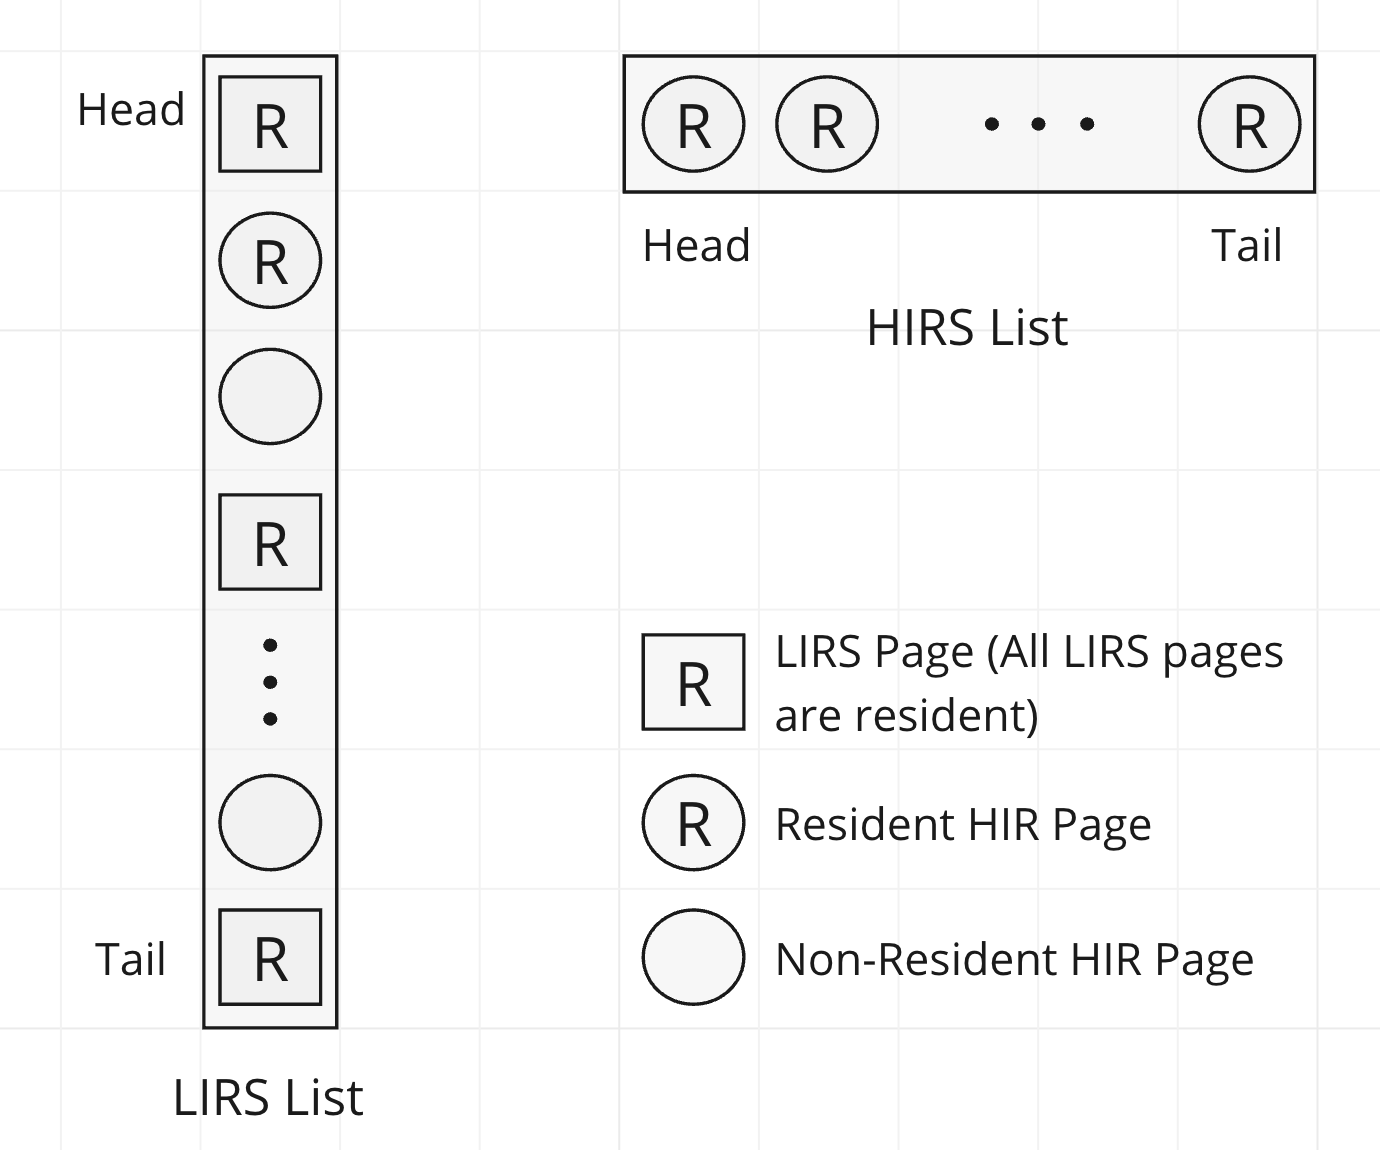
\includegraphics[width=\textwidth]{lirs_and_hirs_lists.png}
        \caption{LIRS and HIRS lists}
        \label{fig:lirs_and_hirs_lists}
    \end{minipage}
    \hfill
\end{figure}

For LIRS cache, we can implement each of the functions as follows:

\begin{itemize}
    \item \textbf{UpdateAccessHistory}(\textit{page}, \textit{tenant}): If it is a LIR page, move it
    to the front of the LIRS list. If it is a HIR page that is on the LIRS list, it is recent, mark it 
    as a LIRS page, and move it to the front of the LIRS list. If it is a HIR page that is not on the LIRS
    list, it is not recent enough to be on the LIRS list, then add it to the front of the HIRS and LIRS lists,
    but marked as a HIR page.
    \item \textbf{AddPageToCache}(\textit{page}, \textit{tenant}, \textit{buffer\_location}): If the page 
    is a non-resident HIR page that is in the LIRS list, move it to the front of the LIRS list, and make it a 
    LIRS page. If the page is not in the LIRS list, add it to the front of the LIRS and HIRS lists, but mark it
    as a HIR page.
    \item \textbf{EvictPage}(\textit{tenant\_to\_evict}): If the HIRS list is not empty, evict the page from the 
    tail of the HIRS list, and update it in the LIRS list to mark it as non-resident HIR page (if it is there). 
    If the HIRS list is empty, evict the page from the tail of the LIRS list.
\end{itemize}

After each operation, LIRS list will be pruned, and the last page of the LIRS list will be moved 
to the HIRS list if needed.

Each operation can be implemented in amortized $O(1)$ time, and the complexity overhead 
of LIRS is low \cite{lirs-article}.

\begin{figure}[htbp]
    \centering
    \begin{minipage}{\linewidth}
    \begin{algorithm}[H]
        \caption{LIRS Cache Eviction Policy}
        \begin{algorithmic}
            \STATE \textbf{function} UpdateAccessHistory(page, tenant):
            \STATE \hspace{\algorithmicindent} \textbf{if} LIRS\_Locations[tenant][page] != \textbf{null} \textbf{then}
            \STATE \hspace{\algorithmicindent} \hspace{\algorithmicindent} pageInLIRS = LIRS\_Locations[tenant][page]
            \STATE \hspace{\algorithmicindent} \hspace{\algorithmicindent} \textbf{if not} pageInLIRS.is\_LIR \textbf{then}
            \STATE \hspace{\algorithmicindent} \hspace{\algorithmicindent} \hspace{\algorithmicindent} pageInLIRS.is\_LIR = \textbf{true}
            \STATE \hspace{\algorithmicindent} \hspace{\algorithmicindent} \hspace{\algorithmicindent} pageInHirs = HIRS\_Locations[tenant][page]
            \STATE \hspace{\algorithmicindent} \hspace{\algorithmicindent} \hspace{\algorithmicindent} HIRS\_List[tenant].Remove(pageInHirs)
            \STATE \hspace{\algorithmicindent} \hspace{\algorithmicindent} \hspace{\algorithmicindent} HIRS\_Locations[tenant][page] = \textbf{null}
            \STATE \hspace{\algorithmicindent} \hspace{\algorithmicindent} \textbf{end if}
            \STATE \hspace{\algorithmicindent} \hspace{\algorithmicindent} LIRS\_List[tenant].\textbf{move\_to\_front}(page)
            \STATE \hspace{\algorithmicindent} \hspace{\algorithmicindent} LIRS\_Locations[tenant][page] = LIRS\_List[tenant].\textbf{head}
            \STATE \hspace{\algorithmicindent} \textbf{else}
            \STATE \hspace{\algorithmicindent} \hspace{\algorithmicindent} pageInHirs = HIRS\_Locations[tenant][page]
            \STATE \hspace{\algorithmicindent} \hspace{\algorithmicindent} HIRS\_List[tenant].\textbf{add\_to\_front}(page)
            \STATE \hspace{\algorithmicindent} \hspace{\algorithmicindent} HIRS\_Locations[tenant][page] = HIRS\_List[tenant].\textbf{head}
            \STATE \hspace{\algorithmicindent} \hspace{\algorithmicindent} LIRS\_List[tenant].\textbf{add\_to\_front}(page) \COMMENT {Marked as HIR}
            \STATE \hspace{\algorithmicindent} \hspace{\algorithmicindent} LIRS\_Locations[tenant][page] = LIRS\_List[tenant].\textbf{head}
            \STATE \hspace{\algorithmicindent} \textbf{end if}
            \STATE \textbf{end function}
            \STATE
            \STATE \textbf{function} AddPageToCache(page, tenant, buffer\_location):
            \STATE \hspace{\algorithmicindent} \textbf{if} LIRS\_Locations[tenant][page] != \textbf{null} \textbf{then}
            \STATE \hspace{\algorithmicindent} \hspace{\algorithmicindent} pageInLirs = LIRS\_Locations[tenant][page]
            \STATE \hspace{\algorithmicindent} \hspace{\algorithmicindent} pageInLirs.is\_LIR = \textbf{true}
            \STATE \hspace{\algorithmicindent} \hspace{\algorithmicindent} LIRS\_List[tenant].\textbf{move\_to\_front}(page)
            \STATE \hspace{\algorithmicindent} \hspace{\algorithmicindent} LIRS\_Locations[tenant][page] = LIRS\_List[tenant].\textbf{head}
            \STATE \hspace{\algorithmicindent} \textbf{else}
            \STATE \hspace{\algorithmicindent} \hspace{\algorithmicindent} HIRS\_List[tenant].\textbf{add\_to\_front}(page)
            \STATE \hspace{\algorithmicindent} \hspace{\algorithmicindent} HIRS\_Locations[tenant][page] = HIRS\_List[tenant].\textbf{head}
            \STATE \hspace{\algorithmicindent} \hspace{\algorithmicindent} LIRS\_List[tenant].\textbf{add\_to\_front}(page) \COMMENT {Marked as HIR}
            \STATE \hspace{\algorithmicindent} \hspace{\algorithmicindent} LIRS\_Locations[tenant][page] = LIRS\_List[tenant].\textbf{head}
            \STATE \hspace{\algorithmicindent} \textbf{end if}
            \STATE \textbf{end function}

            \STATE
            \STATE \textbf{function} EvictPage(tenant\_to\_evict):
            \STATE \hspace{\algorithmicindent} \textbf{if} \textbf{not} HIRS\_List[tenant\_to\_evict].\textbf{empty}() \textbf{then}
            \STATE \hspace{\algorithmicindent} \hspace{\algorithmicindent} pageInHirs = HIRS\_List[tenant\_to\_evict].\textbf{remove\_from\_tail}()
            \STATE \hspace{\algorithmicindent} \hspace{\algorithmicindent} HIRS\_Locations[tenant\_to\_evict][pageInHirs] = \textbf{null}
            \STATE \hspace{\algorithmicindent} \hspace{\algorithmicindent} \textbf{if} LIRS\_Locations[tenant\_to\_evict][pageInHirs] != \textbf{null} \textbf{then}
            \STATE \hspace{\algorithmicindent} \hspace{\algorithmicindent} \hspace{\algorithmicindent} pageInLirs = LIRS\_Locations[tenant\_to\_evict][pageInHirs]
            \STATE \hspace{\algorithmicindent} \hspace{\algorithmicindent} \hspace{\algorithmicindent} pageInLirs.is\_LIR = \textbf{false}
            \STATE \hspace{\algorithmicindent} \hspace{\algorithmicindent} \textbf{end if}
            \STATE \hspace{\algorithmicindent} \hspace{\algorithmicindent} \textbf{return} pageInHirs
            \STATE \hspace{\algorithmicindent} \textbf{else}
            \STATE \hspace{\algorithmicindent} \hspace{\algorithmicindent} pageInLirs = LIRS\_List[tenant\_to\_evict].\textbf{remove\_from\_tail}()
            \STATE \hspace{\algorithmicindent} \hspace{\algorithmicindent} LIRS\_Locations[tenant\_to\_evict][pageInLirs] = \textbf{null}
            \STATE \hspace{\algorithmicindent} \hspace{\algorithmicindent} \textbf{return} pageInLirs
            \STATE \hspace{\algorithmicindent} \textbf{end if}
            \STATE \textbf{end function}
        \end{algorithmic}
    \end{algorithm}
    \caption{LIRS Cache Eviction Policy}
    \label{fig:lirs}
    \end{minipage}
\end{figure}

\newpage

After each function, \textbf{UpdateAccessHistory}, \textbf{AddPageToCache}, and \textbf{EvictPage} 
finishes, we will call \textbf{PruneLIRSList}, and \textbf{MoveLIRSTailToHIRSIfNecessary} with the 
given tenant.

\begin{figure}[htbp]
    \centering
    \begin{minipage}{\linewidth}
    \begin{algorithm}[H]
        \begin{algorithmic}
            \STATE \textbf{function} PruneLIRSList(tenant):
            \STATE \hspace{\algorithmicindent} \textbf{while} \textbf{not} LIRS\_List[tenant].\textbf{empty}() \textbf{and} \textbf{not} LIRS\_List[tenant].\textbf{tail}.is\_LIR \textbf{do}
            \STATE \hspace{\algorithmicindent} \hspace{\algorithmicindent} pageInLirs = LIRS\_List[tenant].\textbf{remove\_from\_tail}()
            \STATE \hspace{\algorithmicindent} \hspace{\algorithmicindent} LIRS\_Locations[tenant][pageInLirs] = \textbf{null}
            \STATE \hspace{\algorithmicindent} \textbf{end while}
            \STATE \textbf{end function}
            \STATE
            \STATE \textbf{function} MoveLIRSTailToHIRSIfNecessary(tenant):
            \STATE \hspace{\algorithmicindent} tenantUsedCache = LIRS\_List[tenant].\textbf{number\_of\_LIRS\_pages}() + HIRS\_List[tenant].\textbf{size}()
            \STATE \hspace{\algorithmicindent} \textbf{if} LIRS\_List[tenant].\textbf{number\_of\_LIRS\_pages}() / tenantUsedCache $>$ LIRS\_Threshold \textbf{then}
            \STATE \hspace{\algorithmicindent} \hspace{\algorithmicindent} page = LIRS\_List[tenant].\textbf{remove\_from\_tail}()
            \STATE \hspace{\algorithmicindent} \hspace{\algorithmicindent} LIRS\_Locations[tenant][page] = \textbf{null}
            \STATE \hspace{\algorithmicindent} \hspace{\algorithmicindent} page.is\_LIR = \textbf{false}
            \STATE \hspace{\algorithmicindent} \hspace{\algorithmicindent} HIRS\_List[tenant].\textbf{add\_to\_front}(page)
            \STATE \hspace{\algorithmicindent} \hspace{\algorithmicindent} HIRS\_Locations[tenant][page] = HIRS\_List[tenant].\textbf{head}
            \STATE \hspace{\algorithmicindent} \hspace{\algorithmicindent} PruneLIRSList(tenant)
            \STATE \hspace{\algorithmicindent} \textbf{end if}
        \end{algorithmic}
    \end{algorithm}
    \caption{Helper Functions for LIRS Cache Eviction Policy}
    \label{fig:lirs-helper}
    \end{minipage}
\end{figure}

LIRS\_List is a doubly linked list that keeps the pages in the cache that are in the LIRS list.

LIRS\_Locations is a hash map or array that keeps the location of the pages in the LIRS list.

HIRS\_List is a doubly linked list that keeps the pages in the cache that are in the HIRS list.

HIRS\_Locations is a hash map or array that keeps the location of the pages in the HIRS list.

LIRS\_Threshold is a tunable parameter that defines the ratio of the number of LIRS pages with 
respect to the total number of pages in the cache.

In LIRS\_List, a counter of the number of LIRS pages is maintained, this counter is updated after 
each operation, and it is used allow $O(1)$ computation of \textbf{number\_of\_LIRS\_pages}()

\subsection{LRFU}

The Least Recently/Frequently Used (LRFU) is a spectrum of cache eviction policies between LRU and 
LFU. 

It associates Combined Recency and Frequency (CRF) value to each page, that quantifies the likelyhood
of a page to be accessed in the near future. Each reference to a page contributes to the CRF value of
the page, and this contribution is determined by a \textit{weighting function} $\mathcal{F}(x)$ where 
$x$ is the number of accesses since the last reference to the page \cite{lrfu-article}.

The CRF value of a page $p$ at time $t_{base}$ is defined as:

$$
\text{CRF}(p, t_{base}) = \sum_{i = 1}^{k} \mathcal{F}(t_{base} - t_{p_i})
$$

where $\mathcal{F}(x)$ is the \textit{weighting function}, $\{ t_{p_1}, t_{p_2}, \ldots, t_{p_k} \}$ are the 
access times of the page $p$ and $t_{p_1} < t_{p_2} < \ldots < t_{p_k}$ \cite{lrfu-article}.

If $\mathcal{F}(x) = c$ for all $x$, then LRFU is equivalent to LFU. If 
$\forall i, \mathcal{F}(i) > \sum_{j = i + 1}^{\infty} \mathcal{F}(j)$, then LRFU is equivalent to LRU.

A class of parametric weighting functions $\mathcal{F}(x)$ that satisfy the following properties in 
their extreme cases is $\mathcal{F}(x) = (\frac{1}{2})^{\lambda x}$, here if $\lambda = 0$, then LRFU is
equivalent to LFU, and if $\lambda = 1$, then LRFU is equivalent to LRU \cite{lrfu-article}. 

An interesting property of the \textit{weighting function} $\mathcal{F}(x)$ is that 
$\mathcal{F}(x+y) = \mathcal{F}(x) \cdot \mathcal{F}(y)$ \cite{lrfu-article}, which allows to update the CRF value of a 
page in a simpler way after each access as follows:

$$
\text{CRF}(p, t_{p_k}) = \mathcal{F}(0) + \mathcal{F}(t_{p_k} - t_{p_{k-1}}) \cdot \text{CRF}(p, t_{p_{k-1}})
$$

Using this, only the last CRF value and the last access time of each page need to be maintained, and it 
is simple to keep it updated after each access.

Since the LRFU policy replaces the page with the smallest CRF value, it is important to keep the pages 
sorted by CRF value, however, the CRF value of a page changes over time. Fortunately, with 
$\mathcal{F}(x) = (\frac{1}{2})^{\lambda x}$, the relative order of two blocks does not change until 
either of them is accessed. Therefore, if $\text{CRF}(p_1, t) < \text{CRF}(p_2, t)$ and neither 
$p_1$ nor $p_2$ have been accessed since $t$, then $\text{CRF}(p_1, t') < \text{CRF}(p_2, t')$
for all $t' \geq t$ \cite{lrfu-article}.

In order to implement LRFU cache, we can use a min-heap to easily evict the page with the smallest 
CRF value.

Time is measured as logical time, and it is incremented after each access. It is possible to keep 
current time per tenant or a global time, the difference is small in practice, we used a global time 
since it showed better results.

For LRFU cache, we can implement each of the functions as follows:

\begin{itemize}
    \item \textbf{UpdateAccessHistory}(\textit{page}, \textit{tenant}): Update the CRF value of the page after each access using the formula above, and heapify.
    \item \textbf{AddPageToCache}(\textit{page}, \textit{tenant}, \textit{buffer\_location}): Add the page to the heap with the CRF value of the page.
    \item \textbf{EvictPage}(\textit{tenant\_to\_evict}): Remove the page with the smallest CRF value from the heap, and return it.
\end{itemize}

\newpage

\begin{figure}[htbp]
    \centering
    \begin{minipage}{\linewidth}
    \begin{algorithm}[H]
        \caption{LRFU Cache Eviction Policy}
        \begin{algorithmic}
            \STATE \textbf{function} UpdateAccessHistory(page, tenant):
            \STATE \hspace{\algorithmicindent} pageInHeap = HeapLocations[tenant][page]
            \STATE \hspace{\algorithmicindent} pageInHeap.CRF = F(0) + F(currentTime - page.lastAccessTime) * pageInHeap.CRF
            \STATE \hspace{\algorithmicindent} pageInHeap.lastAccessTime = currentTime
            \STATE \hspace{\algorithmicindent} Heap[tenant].\textbf{heapify}(pageInHeap)
            \STATE \textbf{end function}
            \STATE
            \STATE \textbf{function} AddPageToCache(page, tenant, buffer\_location):
            \STATE \hspace{\algorithmicindent} page.CRF = F(0)
            \STATE \hspace{\algorithmicindent} page.lastAccessTime = currentTime
            \STATE \hspace{\algorithmicindent} Heap[tenant].\textbf{add}(page)
            \STATE \hspace{\algorithmicindent} HeapLocations[tenant][page] = page
            \STATE \textbf{end function}

            \STATE
            \STATE \textbf{function} EvictPage(tenant\_to\_evict):
            \STATE \hspace{\algorithmicindent} pageToEvict = Heap[tenant\_to\_evict].\textbf{remove\_min}()
            \STATE \hspace{\algorithmicindent} HeapLocations[tenant\_to\_evict][pageToEvict] = \textbf{null}
            \STATE \hspace{\algorithmicindent} \textbf{return} pageToEvict
            \STATE \textbf{end function}

            \STATE
            \STATE \textbf{function} F(x):
            \STATE \hspace{\algorithmicindent} \textbf{return} $(\frac{1}{2})^{\lambda x}$
            \STATE \textbf{end function}
        \end{algorithmic}
    \end{algorithm}
    \caption{LRFU Cache Eviction Policy}
    \label{fig:lrfu}
    \end{minipage}
\end{figure}

Heap is a min-heap that keeps the pages in the cache, and it is sorted by the CRF value of the pages.

HeapLocations is a hash map or array that keeps the location of the pages in the heap.

$\lambda$ is a tunable parameter that defines the weighting function $\mathcal{F}(x)$.

currentTime is a logical time that is incremented after each access.

\subsection{Bélády's Optimal Algorithm}

Bélády's Optimal Algorithm or the clairvoyant algorithm is the theoretical optimal cache eviction
policy, it evicts the page that will be accessed the farthest in the future \cite{lecture-notes-1} 
\cite{lecture-notes-2} \cite{article-for-belady-ref-1}.

This is an offline policy, it needs to know the future accesses to the pages, therefore it is not
practical for real-world applications, it is used here only as a benchmark to compare the performance 
of other cache eviction policies, and see how close they are to the optimal policy.




\cleardoublepage

\chapter{Expermients and Methodology}

\section{Introduction}

This section describes the experiments and methodology used to evaluate the proposed solutions. 
The experiments were conducted on two different datasets: BrightKite and CitiBike, which are 
real-world datasets, and we included a synthetic dataset for parameter tuning.

\section{Datasets}

\subsection{BrightKite Data}

\subsubsection{Overview}

BrightKite was a location-based social network where users shared their locations by checking in at 
different places.

The dataset contains check-ins from users, and each check-in contains the user's ID, the location's ID, 
the timestamp, and the location's geographical coordinates.

BrightKite data was used by Thodoris Lykouris and Sergei Vassilvitskii in their paper "Competitive 
Caching with Machine Learned Advice" \cite{datasets-reference} and the dataset is publicly available
at \cite{brightkite-data}.

From this dataset, we created multiple instances of the caching problem, by considering each user 
as a tenant for our multi-tenant caching problem, location IDs as items or pages to be cached, and 
check-ins as item or page accesses. 

\subsubsection{Processing}

Similar to the work done by Thodoris Lykouris and Sergei Vassilvitskii in \cite{datasets-reference},
we selected the top users where the optimal cache algorithm (Belady's or clairvoyant) had more cache 
faults, to select the most challenging users from the dataset.

Then we created 6 instances of the multi-tenant caching problem, by considering each of the most 
challenging users as a tenant, the locations as items to be cached, and the check-ins as item accesses.

We took 36 most challenging users from the dataset, and created 6 instances of the multi-tenant caching
problem, two of them with 4 tenants, two with 5 tenants, one with 8 tenants, and one with 10 tenants.

Information of the selected users, with number of accesses, number of unique items, and number of cache
faults for the optimal cache algorithm (with cache size equal to 50), rank and user ID, is shown in
Appendix \ref{appendix:brightike-top-36-users}.

The number of accesses per user is from 1300 to 2100, with most of them having 2100. The number of
unique items per user is from 300 to 1300, with many of them having around 600. The number of cache
faults for the optimal cache algorithm is from 10 to 164, with most of them having around 20 or 30.

The cache size recommendations for each tenant started at 40 and kept increasing by 10 until 
the number of extra cache faults for the optimal cache algorithm using a buffer size of the 
recommendation was less than 40.

The number of extra cache faults is the number of cache faults minus the number of unique items accessed, 
since the first access of each item is always a cache fault.

\subsection{CitiBike Data}

\subsubsection{Overview}

CitiBike is a popular bike-sharing service in New York City. We consider citibike trip histories, 
in which each ride is a cache item access. Experiments were made with monthly data from 2023, 
the dataset is publicly available at \cite{citibike-data}.

The dataset contains information about each trip, the start and end station IDs, if the bike
was electric or classic, if the rider is a member or a casual rider, 
the start date and time that was used to sort the data, and more information not used in the 
experiments.

CitiBike data was also used by Thodoris Lykouris and Sergei Vassilvitskii in their paper "Competitive 
Caching with Machine Learned Advice" \cite{datasets-reference}.

We made artificial tenants by considering if the bike was electric or classic, and if the rider 
was a member or a casual rider, therefore we have 4 tenants: electric members, electric casuals,
classic members, and classic casuals.

\subsubsection{Processing}

We made three experiments: 

\begin{itemize}
    \item In the first one, we considered the pair (start\_station\_id, end\_station\_id) to be 
    the items to be cached, so that two trips are only considered the same if they have the 
    same start and end stations.
    \item In the second one, we numbered start stations from 1 to the number of unique start 
    stations, and end stations from 1 to the number of unique end stations, and then considered 
    the pair \(\left(\lfloor \frac{\text{start\_station\_rank}}{5} \rfloor, \lfloor \frac{\text{end\_station\_rank}}{5} \rfloor\right)\) 
    to be the items to be cached.
    \item In the third one, we considered the start station ID to be the item to be cached.
\end{itemize}

The number of unique items and number of accesses in each experiment is shown on the following tables.

\begin{table}[ht]
    \centering
    \small
    \caption{Summary per tenant in the CitiBike experiment 1.}
    \csvautotabular{data/citibike_exp_1_case_2_summary.csv}
    \label{tab:citibike-exp-1-case-2-summary}
\end{table}

\begin{table}[ht]
    \centering
    \small
    \caption{Summary per tenant in the CitiBike experiment 2.}
    \csvautotabular{data/citibike_exp_2_case_3_summary.csv}
    \label{tab:citibike-exp-2-case-3-summary}
\end{table}

\begin{table}[ht]
    \centering
    \small
    \caption{Summary per tenant in the CitiBike experiment 3.}
    \csvautotabular{data/citibike_exp_3_case_4_summary.csv}
    \label{tab:citibike-exp-3-case-4-summary}
\end{table}

% \newpage

The cache size recommendations for each tenant started at 5000, 2000, and 50 in the first, 
second, and third experiments, respectively, and kept increasing by 1000, 400, and 10 until 
the extra cache fault ratio for the optimal cache algorithm using a buffer size of the 
recommendation was less than 20\%, 10\%, and 5\%, respectively.

The extra cache fault ratio is the number of extra cache faults divided by the number of extra 
accesses, where the number of extra cache faults is the number of cache faults minus the number 
of unique items accessed, and the number of extra accesses is the number of accesses minus the 
number of unique items accessed.

\subsection{Random Data}

\subsubsection{Overview}

Random data was used for hyperparameter tuning, testing, and validation of the algorithms, 
but not in the experiments.

It has been shown that when the probability distribution of the data access pattern is constant 
over time, LFU yields the highest performance \cite{lfu-highest-perf-zipf} 
\cite{lfu-highest-perf-inproc} \cite{tiny-lfu}. Therefore, we did not generate data using only 
one probability distribution, as this would favor LFU and not take into account the problem of 
changing access patterns over time.

\subsubsection{Generation}

To generate random data, we used the following probability distributions:

\begin{itemize}
    \item Zipfian distribution, since a popular assumption is that cache workloads follow it 
    \cite{zipf-dist-cache-1} \cite{zipf-dist-cache-2} \cite{zipf-dist-cache-3} 
    \cite{lfu-highest-perf-zipf}.
    \item Pareto distribution, since it has been shown that storage and internet traffic traces 
    are well modeled by it \cite{pareto-dist-workload} \cite{pareto-dist-workload-2} 
    \cite{pareto-dist-workload-3}.
    \item Normal distribution; we used it less than the other distributions since it is not 
    commonly used in cache workloads, but it was used in \cite{memory-aware-buffer-pool-manager}.
    \item Uniform distribution; we used it less than the other distributions since it is not 
    commonly used in cache workloads, but it was used in \cite{memory-aware-buffer-pool-manager}.
\end{itemize}

To address the problem of changing access patterns over time, in some cases, we generated data 
using one distribution for a period of time, and then changed the distribution to another one. 
In many cases, the distribution was the same, but we renumbered the most accessed items.

To address the problem of correlated accesses, in some cases, when generating data for the 
tenants, we generated correlated accesses to some items, causing them to be accessed together 
during certain periods of time.

To handle multi tenancy, in some cases we randomly merged the data of the tenants, and in 
other cases we splitted the data of each tenant into chunks, and then randomly merged the
chunks.

\section{Testing and Validation}

\subsection{Data Validation}

In order to ensure the integrity of the data, we validated each case for the experiments and 
the randomly generated data.

For each case, we checked that each tenant had the correct number of accesses and the correct 
number of unique items, both by script and by visually plotting the data to ensure it was 
correctly generated.

Additional integrity checks related to buffer sizes, priority levels, and tenant information 
were also performed.

\subsection{Algorithm Validation}

In order to validate the algorithms, we simulated the cache eviction process for each case, 
keeping track of the cache state and the cache faults, and performing integrity checks related 
to the cache state, cache hits, and faults.

Checks related to the tenant selection policy were performed to ensure that each tenant had at 
least the minimum buffer size promised at any time, did not exceed the maximum buffer size 
promised at any time, and was selected according to the tenant selection policy.

Additional checks related to the cache eviction policy were performed to ensure that the 
eviction policy was correctly implemented and worked as expected.

\section{Experiments}

\subsection{Overview}

For each experiment type, we ran each cache eviction policy, using the fault ratio with 
cache used tenant selection policy on the following datasets:

\begin{itemize}
    \item BrightKite experiment data.
    \item CitiBike 1st experiment data.
    \item CitiBike 2nd experiment data.
    \item CitiBike 3rd experiment data.
\end{itemize}

The minimum buffer size per tenant was set to 40\% of the cache size recommendation, and the
maximum buffer size per tenant was set to 250\% of the cache size recommendation for the 
BrightKite experiment, and 220\% of the cache size recommendation for the CitiBike experiments.

The total buffer size was set to 80\% of the sum of the cache size recommendations for each 
tenant.

\subsection{Hit Ratio Per Cache Size Experiment}

In the hit ratio per cache size experiment, we ran the cache eviction policies with 10 different
cache sizes, and computed the hit ratio for each cache size and tenant.

The cache sizes used per experiment were:

\begin{itemize}
    \item BrightKite experiment: 50, 75, 100, 125, 150, 175, 200, 225, 250, 275.
    \item CitiBike 1st experiment: 4000, 8000, 12000, 16000, 20000, 24000, 28000, 32000, 36000, 40000.
    \item CitiBike 2nd experiment: 3000, 6000, 9000, 12000, 15000, 18000, 21000, 24000, 27000, 30000.
    \item CitiBike 3rd experiment: 200, 400, 600, 800, 1000, 1200, 1400, 1600, 1800, 2000.
\end{itemize}

These sizes were selected based on the number of unique items and the number of accesses, as 
well as the number of cache faults for the optimal cache algorithm.

The cache size recommendations for each tenant were scaled based on the total buffer size to 
keep the total buffer size at 80\% of the sum of the cache size recommendations for each tenant.

Minimum and maximum buffer sizes were also scaled based on the cache size recommendations.

\subsection{Fault Score Experiment}

In the fault score experiment, we ran the cache eviction policies in the BrightKite experiment 
and in the three CitiBike experiments, and computed the penalty function score (fault score) 
for each cache eviction policy in each experiment.

The cache size recommendations for each tenant were set as described in the dataset processing 
section.

Minimum buffer sizes, maximum buffer sizes, and total buffer size were set as described in 
the experiments overview section.

\cleardoublepage

\chapter{Results}

\section{Hit Ratio Per Cache Size Experiment}

\lipsum[1-3]

\section{Fault Score Experiment}

\lipsum[1-1] \ref{fig:figA-1}

\begin{figure}[H]
    \centering
    \includegraphics[width=0.3  \textwidth]{dummy.png}
    \caption{Lorem ipsum dolor sit amet}
    \label{fig:figA-4}
\end{figure}

\lipsum[1-1] \ref{fig:figB-1}

\begin{figure}[H]
    \centering
    \includegraphics[width=0.3\textwidth]{dummy.png}
    \caption{Lorem ipsum dolor sit amet}
    \label{fig:figB-4}
\end{figure}


\lipsum[1-1] \cite{reference-1}
\lipsum[1-1] \cite{reference-2}


\lipsum[1-1] \cite{reference-3}

\begin{table}[ht!]
    \centering
    \begin{tabular}{c c c}
        \hline
        Column 1 & Column 2 & Column 3 \\
        \hline
        Item 1   & Item 2   & Item 3   \\
    \end{tabular}
    \caption{Lorem ipsum dolor sit amet}
    \label{tab:tabA-4}
\end{table}

\lipsum[1-1] \ref{tab:tabA-1}

\begin{table}[ht!]
    \centering
    \begin{tabular}{c c c}
        \hline
        Column 1 & Column 2 & Column 3 \\
        \hline
        Item 1   & Item 2   & Item 3   \\
    \end{tabular}
    \caption{Lorem ipsum dolor sit amet}
    \label{tab:tabB-4}
\end{table}

\lipsum[1-1] \ref{tab:tabB-1}

\lipsum[1-2]

\cleardoublepage
\nocite{*}
\printbibliography
\addcontentsline{toc}{chapter}{Bibliography}

\cleardoublepage
\appendix
\input{appendix/appendix-list.tex}

\ifodd\value{page}
\else
\newpage
\thispagestyle{empty}
\mbox{}
\fi

\end{document}